\documentclass[twocolumn]{aastex631}

\graphicspath{{/Users/devaldeliwala/classes/physics129/final_project/images/}}

\usepackage{float} % for 'htp' placement
\usepackage{multirow}
\usepackage{amsmath}
\usepackage{hyperref}

\begin{document}

\title{Simulating CMS Calorimeter Response of Electromagnetic Showers}

\author{Deval Deliwala}
\affiliation{University of California, Berkeley}

\shorttitle{Simulating Calorimeter Response of Electromagnetic Showers}
\shortauthors{Deliwala}

\begin{abstract}
Accurate simulation of electromagnetic shower development within the Compact Muon Solenoid (CMS) electromagnetic calorimeter (ECAL) is essential for precise energy measurements in high-energy physics experiments. This study presents a Monte Carlo simulation that models the longitudinal development of electromagnetic showers using a one-dimensional approximation. Phase 1 focuses on simulating the shower profile for 1 GeV incident electrons in a 25 cm lead tungstate (PbWO\(_4\)) calorimeter, validating the simulation against established benchmarks. Phase 2 assesses the detector's linearity and energy resolution by calibrating the energy deposition and examining its dependence on varying incident energies (1, 3, 5, and 10 GeV). Phase 3 involves fitting the energy deposition function to a gamma distribution, extracting parameters that characterize the shower development. Phase 4 explores the detector's performance as a function of calorimeter thickness, investigating the onset of non-linearities in energy response and the scaling of energy resolution. The simulation demonstrates a linear relationship between incident energy and mean energy deposited, as well as a square root scaling of energy resolution with energy, consistent with CMS expectations. These foundational phases establish a framework for further exploration into more complex shower dynamics and detector performance metrics.
\end{abstract}

\section{Introduction}

The accurate measurement of particle energies is a cornerstone of high-energy physics experiments. Electromagnetic calorimeters (ECALs) play a crucial role in detecting and measuring the energy of electrons and photons produced in particle collisions. The CMS ECAL, constructed from lead tungstate (PbWO\(_4\)) crystals, is designed to provide high-resolution energy measurements essential for a wide range of physics analyses, including the identification of Higgs boson decays and searches for new particles.

Understanding the longitudinal development of electromagnetic showers within the ECAL is vital for optimizing its performance and interpreting experimental data. This study employs a Monte Carlo simulation with simplifying assumptions to model the longitudinal distribution of charged particles and photons generated by electromagnetic showers initiated by incident electrons. The work is divided into four primary phases:

\begin{enumerate}
    \item \textbf{Phase 1}: Simulates the one-dimensional longitudinal development for 1 GeV incident electrons, validating the simulation against established benchmarks.
    \item \textbf{Phase 2}: Assesses the detector's linearity and energy resolution across multiple incident energies (1, 3, 5, and 10 GeV).
    \item \textbf{Phase 3}: Fits the energy deposition function to a gamma distribution, extracting parameters that characterize the shower development.
    \item \textbf{Phase 4}: Examines the detector's performance as a function of calorimeter thickness, investigating the onset of non-linearities in energy response and analyzing the scaling of energy resolution.
\end{enumerate}

The results provide insights into the functional dependence of shower development on energy and validate the simulation against established benchmarks.

This paper is structured as follows: Section \ref{sec:ecal} provides a detailed description of the CMS electromagnetic calorimeter. Section \ref{sec:methods} outlines the simulation methods, including the assumptions and computational techniques used in Phases 1 through 4 of the project. Sections \ref{sec:results_phase1} to \ref{sec:results_phase4} present the simulation results for each phase, respectively. Section \ref{sec:conclusion} offers conclusions and discusses future work.

\section{The Electromagnetic Calorimeter}\label{sec:ecal}

The CMS electromagnetic calorimeter is a critical component of the CMS detector at the Large Hadron Collider (LHC). It is designed to measure the energy of electrons and photons with high precision and is composed of approximately 75,848 lead tungstate (PbWO\(_4\)) crystals. These crystals are chosen for their high density, short radiation length, and fast scintillation properties, which are essential for the detection of high-energy particles within a compact volume.

Key features of the CMS ECAL include:

\begin{itemize}
    \item \textbf{Material Composition}: PbWO\(_4\) crystals serve as the active medium, providing a dense material that facilitates the development of electromagnetic showers within a relatively short distance.
    \item \textbf{Geometry and Depth}: The ECAL is segmented into a barrel region and two endcaps, each consisting of multiple layers of crystals. The total depth of the calorimeter is approximately 25 cm, corresponding to several radiation lengths, which is sufficient to contain the majority of electromagnetic showers initiated by high-energy electrons and photons.
    \item \textbf{Readout System}: Each crystal is coupled to a photodetector, typically a photodiode or avalanche photodiode (APD), which converts the scintillation light into an electrical signal. The readout system is designed to handle high rates of particle interactions and provide precise energy measurements.
    \item \textbf{Energy Resolution}: The ECAL achieves excellent energy resolution, which is critical for distinguishing between different particle types and for precise measurements of particle energies. The resolution depends on factors such as the number of crystals, the quality of the scintillation process, and the precision of the readout electronics.
\end{itemize}

Understanding the longitudinal development of electromagnetic showers within the ECAL is essential for optimizing its performance and ensuring accurate energy measurements. This study focuses on simulating this development using a simplified one-dimensional model, laying the groundwork for more comprehensive simulations that account for three-dimensional shower characteristics and additional physical processes.

\section{Methods}\label{sec:methods}

This section outlines the Monte Carlo simulation approach used to model the longitudinal development of electromagnetic showers in the CMS ECAL. The simulation is divided into four phases:

\begin{enumerate}
    \item \textbf{Phase 1}: Simulates the longitudinal distribution for 1 GeV incident electrons.
    \item \textbf{Phase 2}: Assesses the detector's linearity and energy resolution across multiple incident energies.
    \item \textbf{Phase 3}: Fits the energy deposition function to a gamma distribution, extracting parameters that characterize the shower development.
    \item \textbf{Phase 4}: Examines the detector's performance as a function of calorimeter thickness, investigating the onset of non-linearities in energy response and analyzing the scaling of energy resolution.
\end{enumerate}

\subsection{Phase 1: Monte Carlo Simulation of the Charged Particle and Photon Distribution}

The objective of Phase 1 is to develop a Monte Carlo simulation that predicts the longitudinal development of an electromagnetic shower initiated by 1 GeV electrons in a 25 cm lead tungstate (PbWO\(_4\)) calorimeter. The simulation aims to generate plots of the average number of charged particles and photons as a function of the distance from the front face of the calorimeter.

\subsubsection{Simplifying Assumptions}

To make the simulation tractable, several simplifying assumptions are employed. These assumptions deviate from the real-world behavior of electromagnetic showers but allow for a foundational understanding of the shower development process.

\begin{enumerate}
    \item \textbf{Calorimeter Geometry}: The ECAL is modeled as a uniform, one-dimensional crystal of PbWO\(_4\) with a depth of 25 cm. Electrons are assumed to enter the front face of the crystal with a fixed energy of 1 GeV and normal incidence.
    
    \item \textbf{One-Dimensional Shower Development}: Real electromagnetic showers develop in three dimensions, exhibiting both longitudinal and transverse spread. For simplicity, the simulation employs a one-dimensional model, neglecting any transverse spreading of the shower.
    
    \item \textbf{Discrete Bremsstrahlung Processes}: Electrons lose energy primarily through bremsstrahlung. Instead of modeling this as a continuous process, the simulation approximates energy loss as discrete events occurring at random positions along the electron's trajectory. The probability of a bremsstrahlung event occurring within a differential distance \(dx\) is given by:
    \[
    dP = \frac{dN}{N} = - \frac{dx}{X_0}
    \]
    where \(X_0\) is the radiation length of PbWO\(_4\).
    
    \item \textbf{Equal Energy Division in Bremsstrahlung}: Upon a bremsstrahlung event, the energy is equally divided between the outgoing electron and the emitted photon. This is an unrealistic simplification, as the actual bremsstrahlung spectrum is peaked at low photon energies.
    
    \item \textbf{Constant Ionization Energy Loss}: Charged particles (\(e^+\) and \(e^-\)) lose energy via ionization at a constant rate per centimeter, derived from the PDG's atomic and nuclear properties of PbWO\(_4\). The simulation ignores the Landau distribution of energy loss and the Bragg peak effect as particles come to rest.
    
    \item \textbf{Photon Interactions}: Photons interact primarily through pair production in this simulation. The probability of pair production within a differential distance \(dx\) is:
    \[
    dP = \frac{dx}{\frac{9}{7} X_0}
    \]
    Upon pair production, the resulting electron and positron share the photon's energy equally, and electrons are treated as massless particles.
\end{enumerate}

\subsubsection{Simulation Procedure}

The simulation follows these steps for each event:

\begin{enumerate}
    \item \textbf{Initialization}: Start with a single 1 GeV electron at the front face (\(x = 0\) cm) of the 25 cm PbWO\(_4\) calorimeter.
    
    \item \textbf{Track Management}: Maintain a list of active particles (electrons, positrons, and photons) with their respective energies and positions.
    
    \item \textbf{Energy Loss and Interactions}:
    \begin{itemize}
        \item For each charged particle, determine the distance to the next bremsstrahlung event based on the radiation length \(X_0\).
        \item At each bremsstrahlung event, split the energy equally between the outgoing electron and the emitted photon.
        \item For each photon, determine the distance to the next pair production event using the modified radiation length (\(\frac{9}{7} X_0\)).
        \item At each pair production event, generate an electron-positron pair, each receiving half of the photon's energy.
    \end{itemize}
    
    \item \textbf{Energy Loss via Ionization}: For each charged particle, subtract the ionization energy loss per centimeter from its energy as it traverses the calorimeter. If a particle's energy drops to zero or below, it is removed from the active list.
    
    \item \textbf{Position Update}: Advance the position of each particle based on the distances traveled during interactions and energy loss.
    
    \item \textbf{Event Termination}: Continue the simulation until all particles have either exited the calorimeter or been absorbed due to energy loss.
\end{enumerate}

\subsubsection{Data Collection and Analysis}

For each simulated event, record the positions where charged particles and photons cross planes at specified distances from the front face of the calorimeter. After simulating 1000 events, compute the average number of charged particles and photons crossing each plane. These averages are then plotted as functions of the calorimeter depth, enabling comparison with established benchmarks such as the PDG \textit{Passage of Particles Through Matter} Booklet's Figure 33.20.

\subsubsection{Comparison with PDG Benchmark}

The PDG \textit{Passage of Particles Through Matter} Booklet's Figure 33.20 illustrates the longitudinal development of electromagnetic showers in different materials and for varying incident energies. Specifically, it shows an EGS4 simulation of a 30 GeV electron-induced cascade in iron, with fractional energy deposition per radiation length and the number of electrons and photons crossing planes at radiation length intervals. While the simulation employs a one-dimensional model and PbWO\(_4\) instead of iron, the general features of the shower development, such as the position of the shower maximum and the relative densities of charged particles and photons, are expected to align qualitatively with the PDG benchmarks. Quantitative differences arise due to the simplifying assumptions and differences in material properties and incident energies.

\subsection{Phase 2: Linearity and Energy Resolution of the Detector}

Phase 2 extends the Monte Carlo simulation to evaluate the detector's linearity and energy resolution by analyzing the total energy deposited in the calorimeter across varying incident energies. This phase involves calibrating the detector response and examining the relationship between incident energy and measured energy deposition.

\subsubsection{Energy Deposition and Calibration}

To assess the energy resolution, the simulation tracks the total energy deposited in the calorimeter from each of the 1000 events. The total energy deposition is calculated as the integral of the charged particle density along the entire crystal length, effectively summing the energy lost via ionization. Photons are excluded from this analysis to focus solely on charged particle contributions.

\paragraph{Initial Calibration}

An initial simulation with 1 GeV incident electrons produced a mean energy deposition of 3.027 GeV with a standard deviation of 0.263 GeV. The observed mean was approximately three times the incident energy, likely due to the assumption that ionization energy loss is solely based on distance traveled without energy conservation constraints. To calibrate the detector, the total energy deposition for each event was divided by 3, aligning the mean deposition with the known incident energy. This calibration was consistently effective across multiple incident energies, yielding histogram means within ±0.01 GeV of the expected values.

\subsubsection{Simulation at Multiple Incident Energies}

The calibrated Monte Carlo simulation was run for incident energies of 1, 3, 5, and 10 GeV. For each energy, the average charged particle density as a function of calorimeter depth was computed and plotted on the same graph with distinct colors and a corresponding legend.

\paragraph{Results}

\begin{figure}[htp]
    \centering
    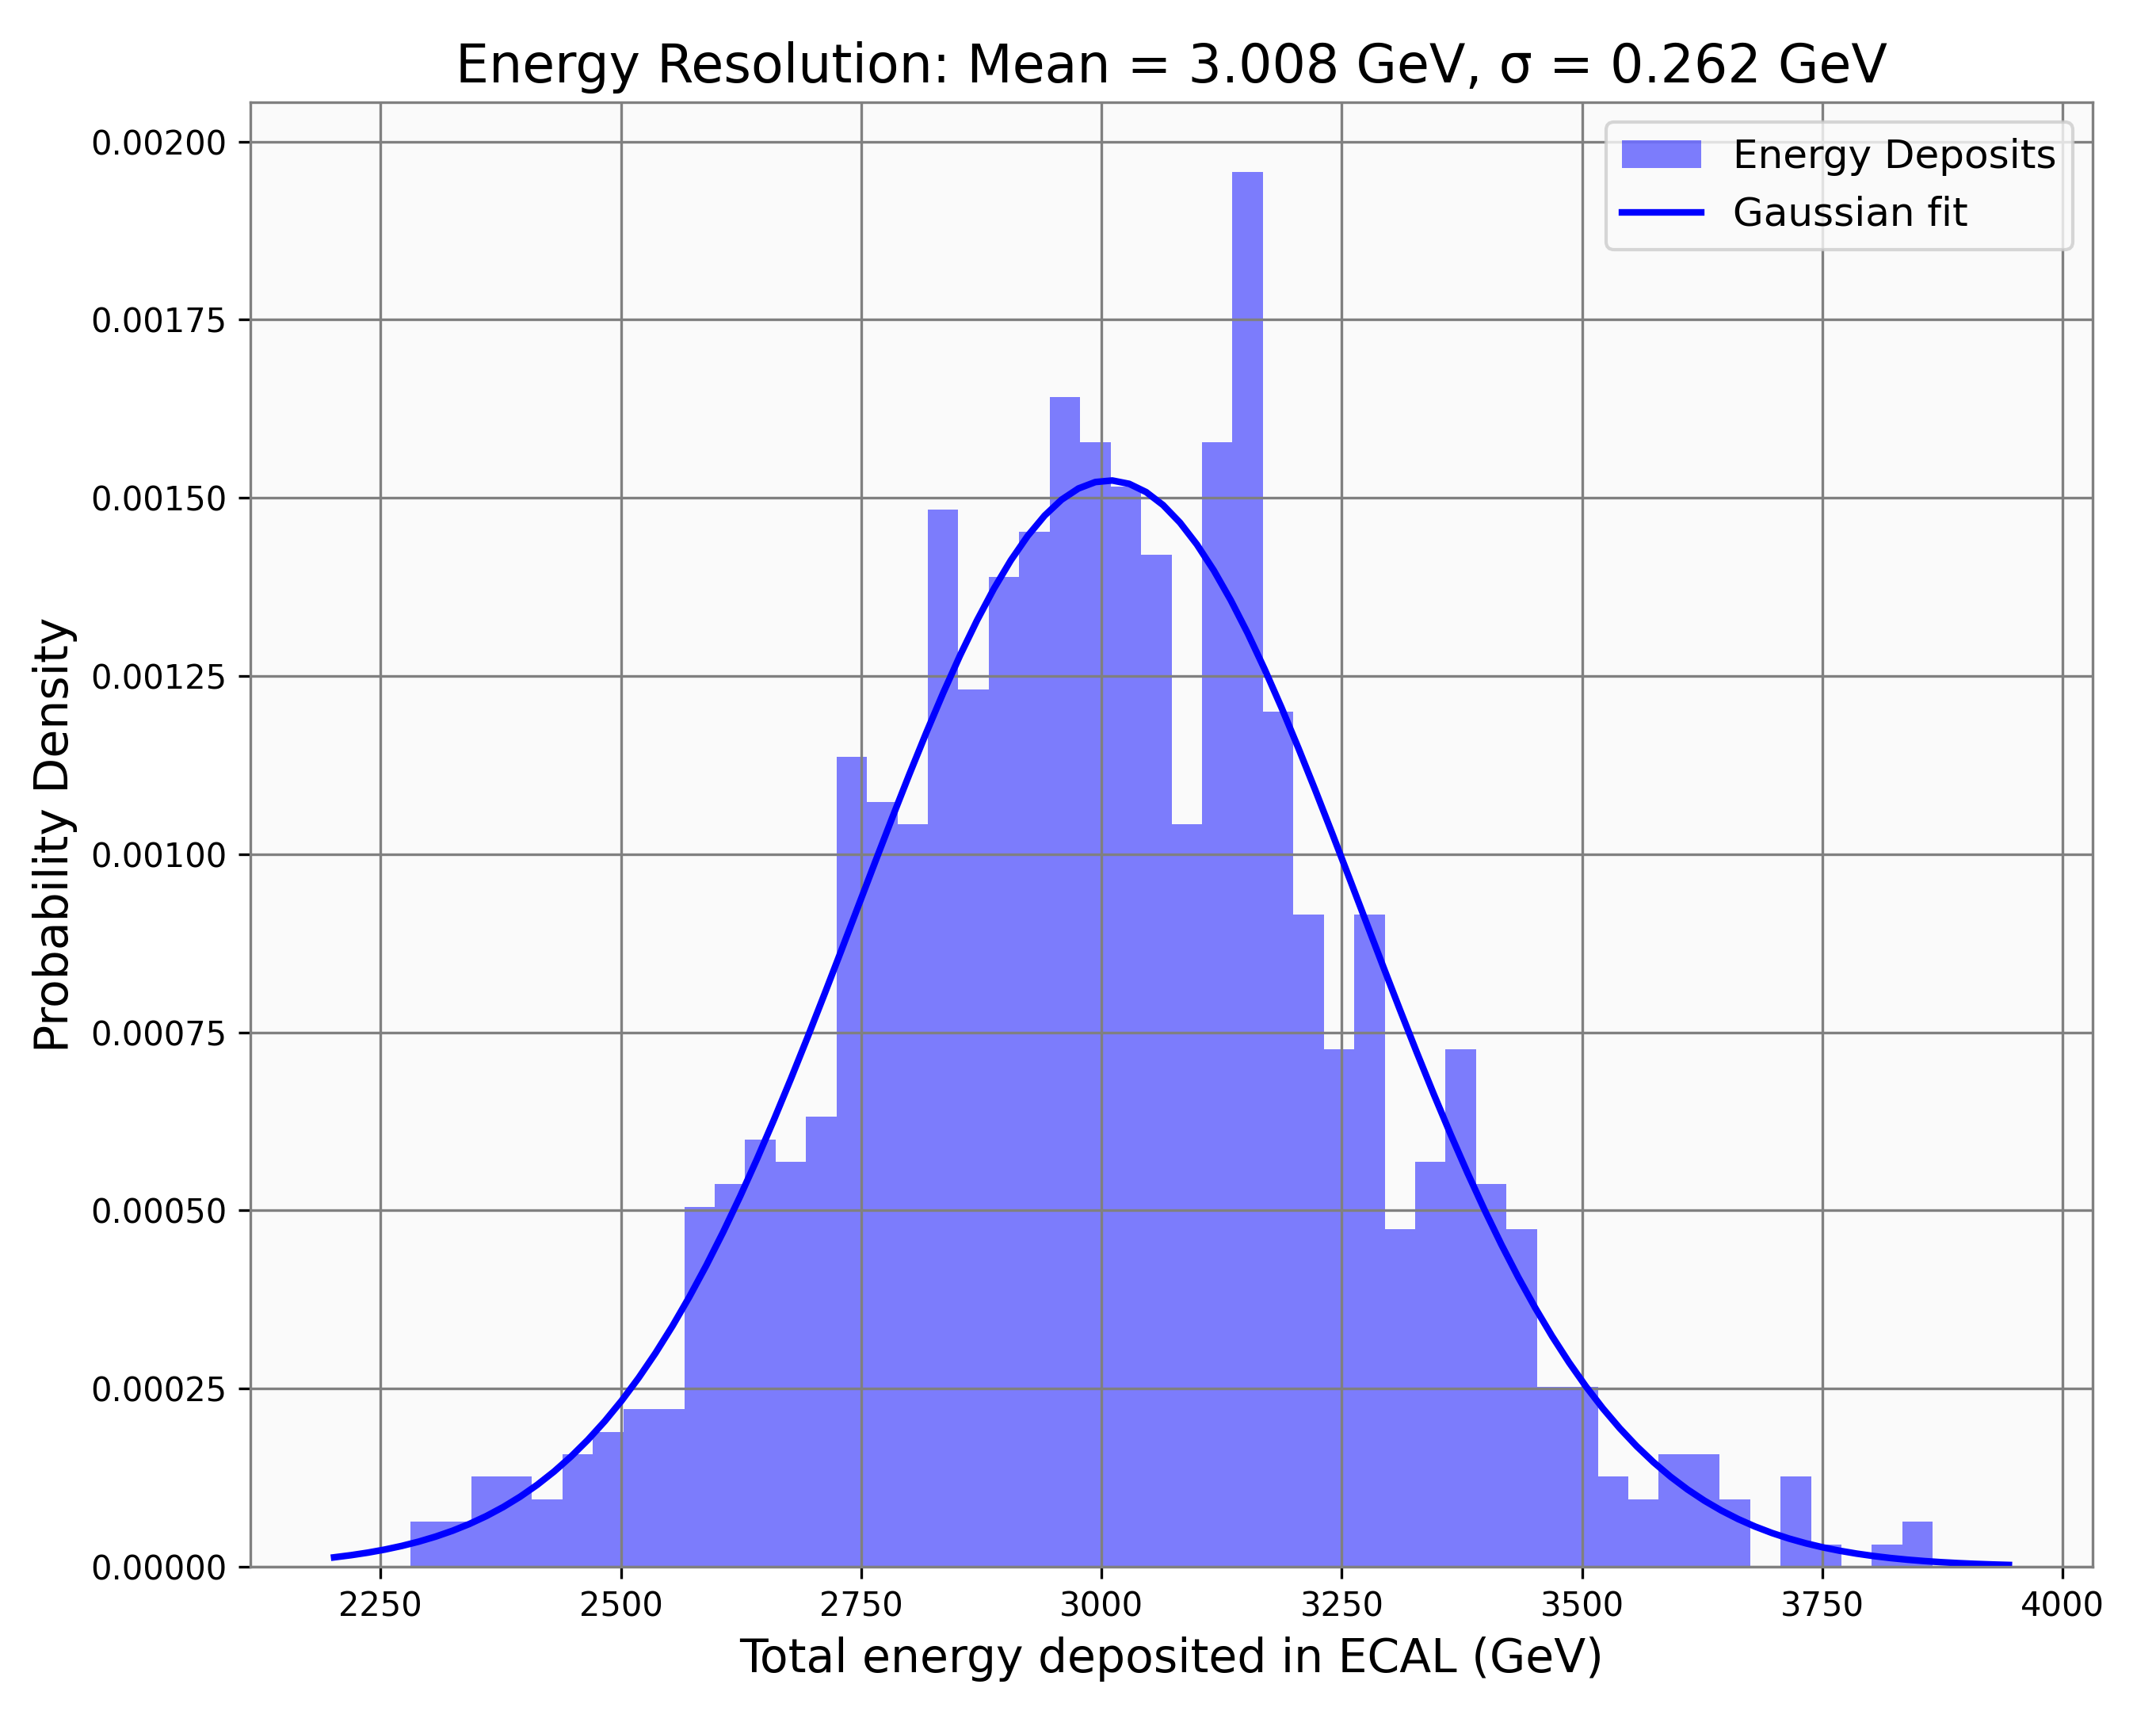
\includegraphics[width=\columnwidth]{part2_a.png}
    \caption{Average number of charged particles as a function of calorimeter depth for incident energies of 1, 3, 5, and 10 GeV. Each curve is color-coded and labeled accordingly. Higher incident energies result in increased average charged particle densities and shifts in the shower maximum depth.}
    \label{fig:charged_particles_multiple_energies}
\end{figure}

As the incident energy increases, the average number of charged particles in the shower increases linearly, while the depth at which the peak number of charged particles occurs shifts deeper into the calorimeter. For example, the peak occurs at approximately 4 cm for 1 GeV and extends to about 6 cm for 10 GeV, corresponding to 4.49 and 6.74 radiation lengths (\(X_0 = 0.89\) cm), respectively. The longitudinal distributions maintain a normal distribution shape, with higher energies resulting in steeper distributions.

\subsubsection{Energy Deposition vs. Incident Energy}

\begin{figure}[htp]
    \centering
    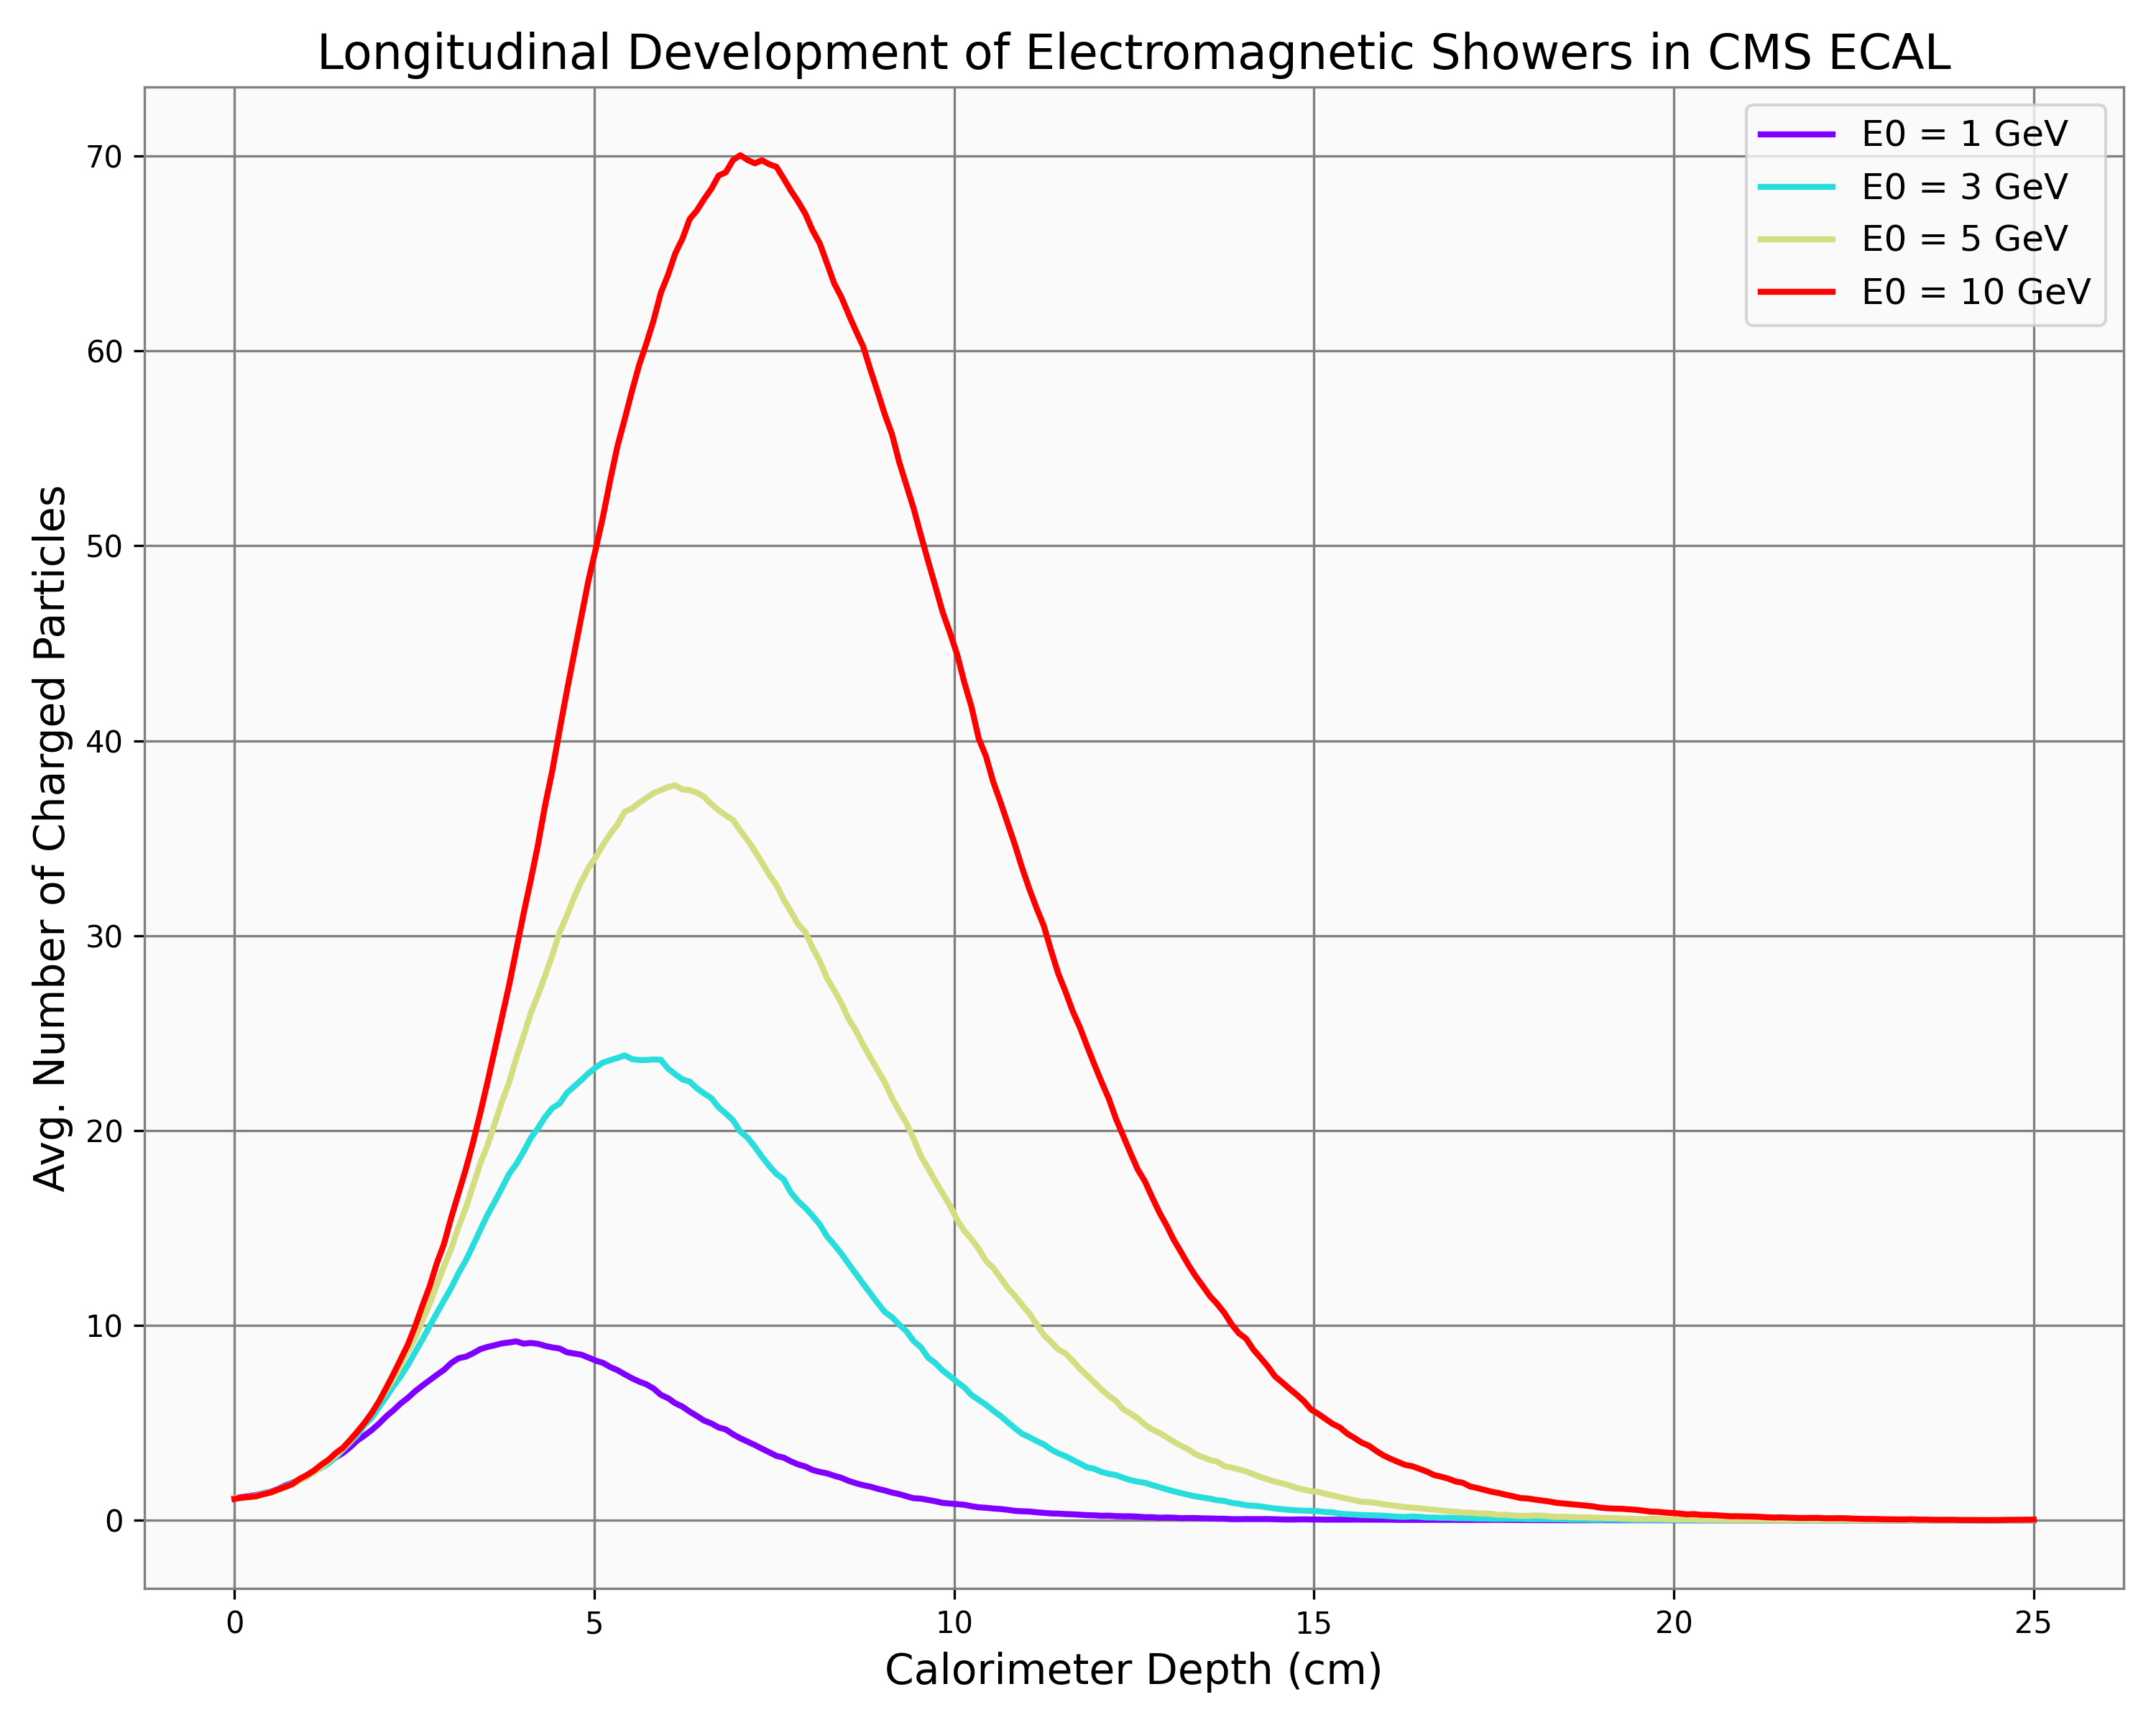
\includegraphics[width=\columnwidth]{part2_b.png}
    \caption{Mean energy deposition in the calorimeter as a function of incident energy. The relationship is perfectly linear, with a calibration factor of 1.00 and an intercept of 0.00, indicating accurate detector calibration under simplifying assumptions.}
    \label{fig:energy_deposition_vs_incident_energy}
\end{figure}

The relationship between the mean energy deposited in the calorimeter and the incident energy was plotted, revealing a perfect linear fit described by \(y = 1.00x + 0.00\). This linearity is a direct consequence of the simplifying assumptions made in the simulation, particularly the proportionality of ionization energy loss to distance traveled and the equal energy sharing in bremsstrahlung processes.

\subsubsection{Energy Resolution Scaling}

\begin{figure}[htp]
    \centering
    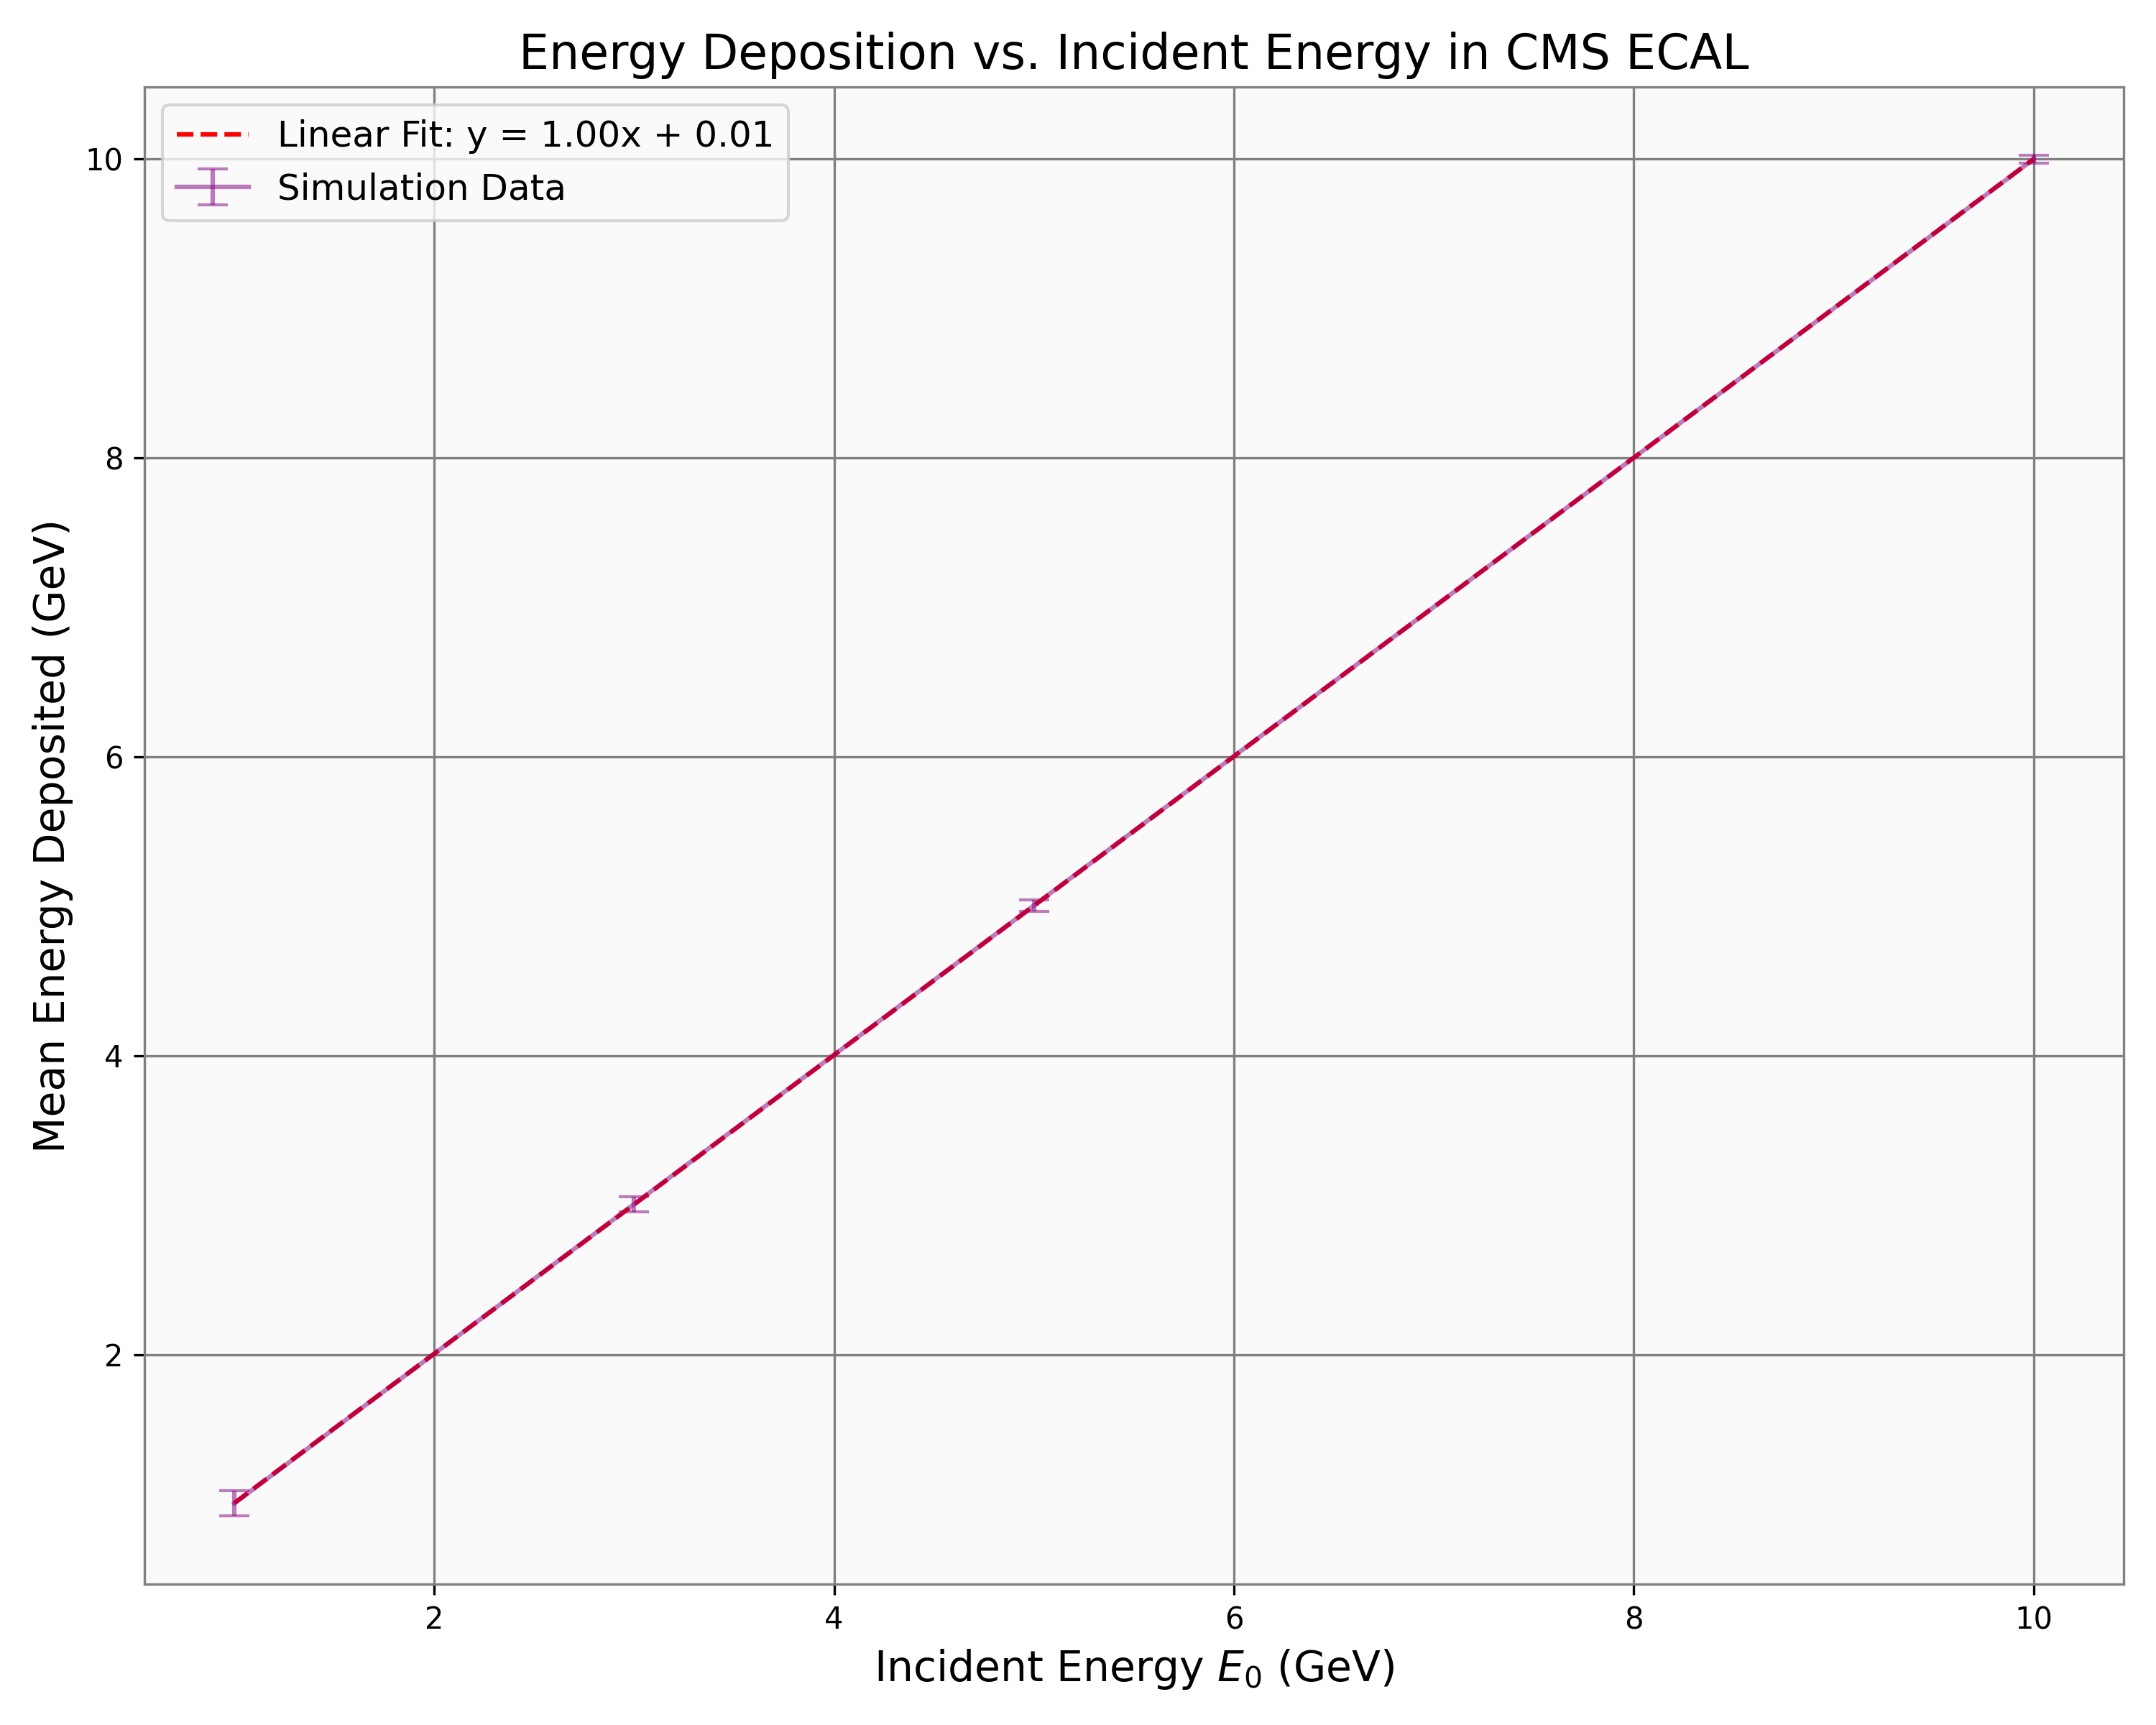
\includegraphics[width=\columnwidth]{part2_c.png}
    \caption{Calorimeter energy resolution (\(\sigma\)) as a function of incident energy. The resolution follows a square root dependence, fitting the relation \(\sigma = 0.09 \sqrt{E_0} - 0.007\), consistent with CMS reports.}
    \label{fig:energy_resolution_vs_energy}
\end{figure}

The energy resolution of the calorimeter was evaluated by plotting the standard deviation of the energy deposition distribution against the incident energy. The resolution follows a square root dependence, best described by the fit \(\sigma = 0.09 \sqrt{E_0} - 0.007\). This functional form is consistent with CMS reports, which typically observe that energy resolution scales as \(\sigma/E \propto \frac{1}{\sqrt{E}}\), reflecting the stochastic nature of the energy deposition processes in the calorimeter.

\subsection{Phase 3: Fitting the Energy Deposition Function}

Phase 3 involves fitting the energy deposition function to a gamma distribution to characterize the shower development. The energy deposition per unit length is modeled by the function:

\[
\frac{dE}{dt} = E_0 b \frac{(bt)^{a-1}e^{-bt}}{\Gamma(a)}
\]

where \(t\) is the dimensionless length scale \(x/X_0\), and \(a, b\) are constants to which the data are fit. Since the simulation tracks the number of charged particles rather than energy, the charged particle density is normalized by the total number of charged particles deposited at 1 GeV, effectively providing a conversion constant from the number of particles to energy in GeV.

\paragraph{Fitted Parameters}

Using data from Phase 2, the parameters \(a\) and \(b\) were extracted for incident energies of 1, 3, 5, and 10 GeV. The results are summarized in Table \ref{tab:fitted_parameters}.

\begin{table}[htp]
    \centering
    \caption{Fitted parameters \(a\) and \(b\) for the energy deposition function at various incident energies.}
    \label{tab:fitted_parameters}
    \begin{tabular}{ccc}
        \hline
        \textbf{E\(_0\) (GeV)} & \textbf{a} & \textbf{b} \\
        \hline
        1 & 0.7991 & 0.0030 \\
        3 & 0.8622 & 0.0032 \\
        5 & 0.8784 & 0.0031 \\
        10 & 0.9400 & 0.0037 \\
        \hline
    \end{tabular}
\end{table}

These parameters indicate how the energy deposition profile evolves with increasing incident energy, reflecting changes in the shower development dynamics within the calorimeter.

\subsection{Phase 4: Linearity and Resolution vs. Calorimeter Thickness}

Phase 4 examines how the performance of the calorimeter changes as a function of its thickness, measured in radiation lengths (\(X_0\)). Specifically, it investigates the onset of non-linearities in the energy response and analyzes how energy resolution scales with calorimeter depth.

\subsubsection{Mean Energy Deposition vs. Incident Energy for Varying Thicknesses}

The simulation was run for calorimeter depths of 5, 10, 15, 20, and 25 \(X_0\), and the mean energy deposition was recorded for incident energies of 1, 3, 5, and 10 GeV.

\begin{figure}[htp]
    \centering
    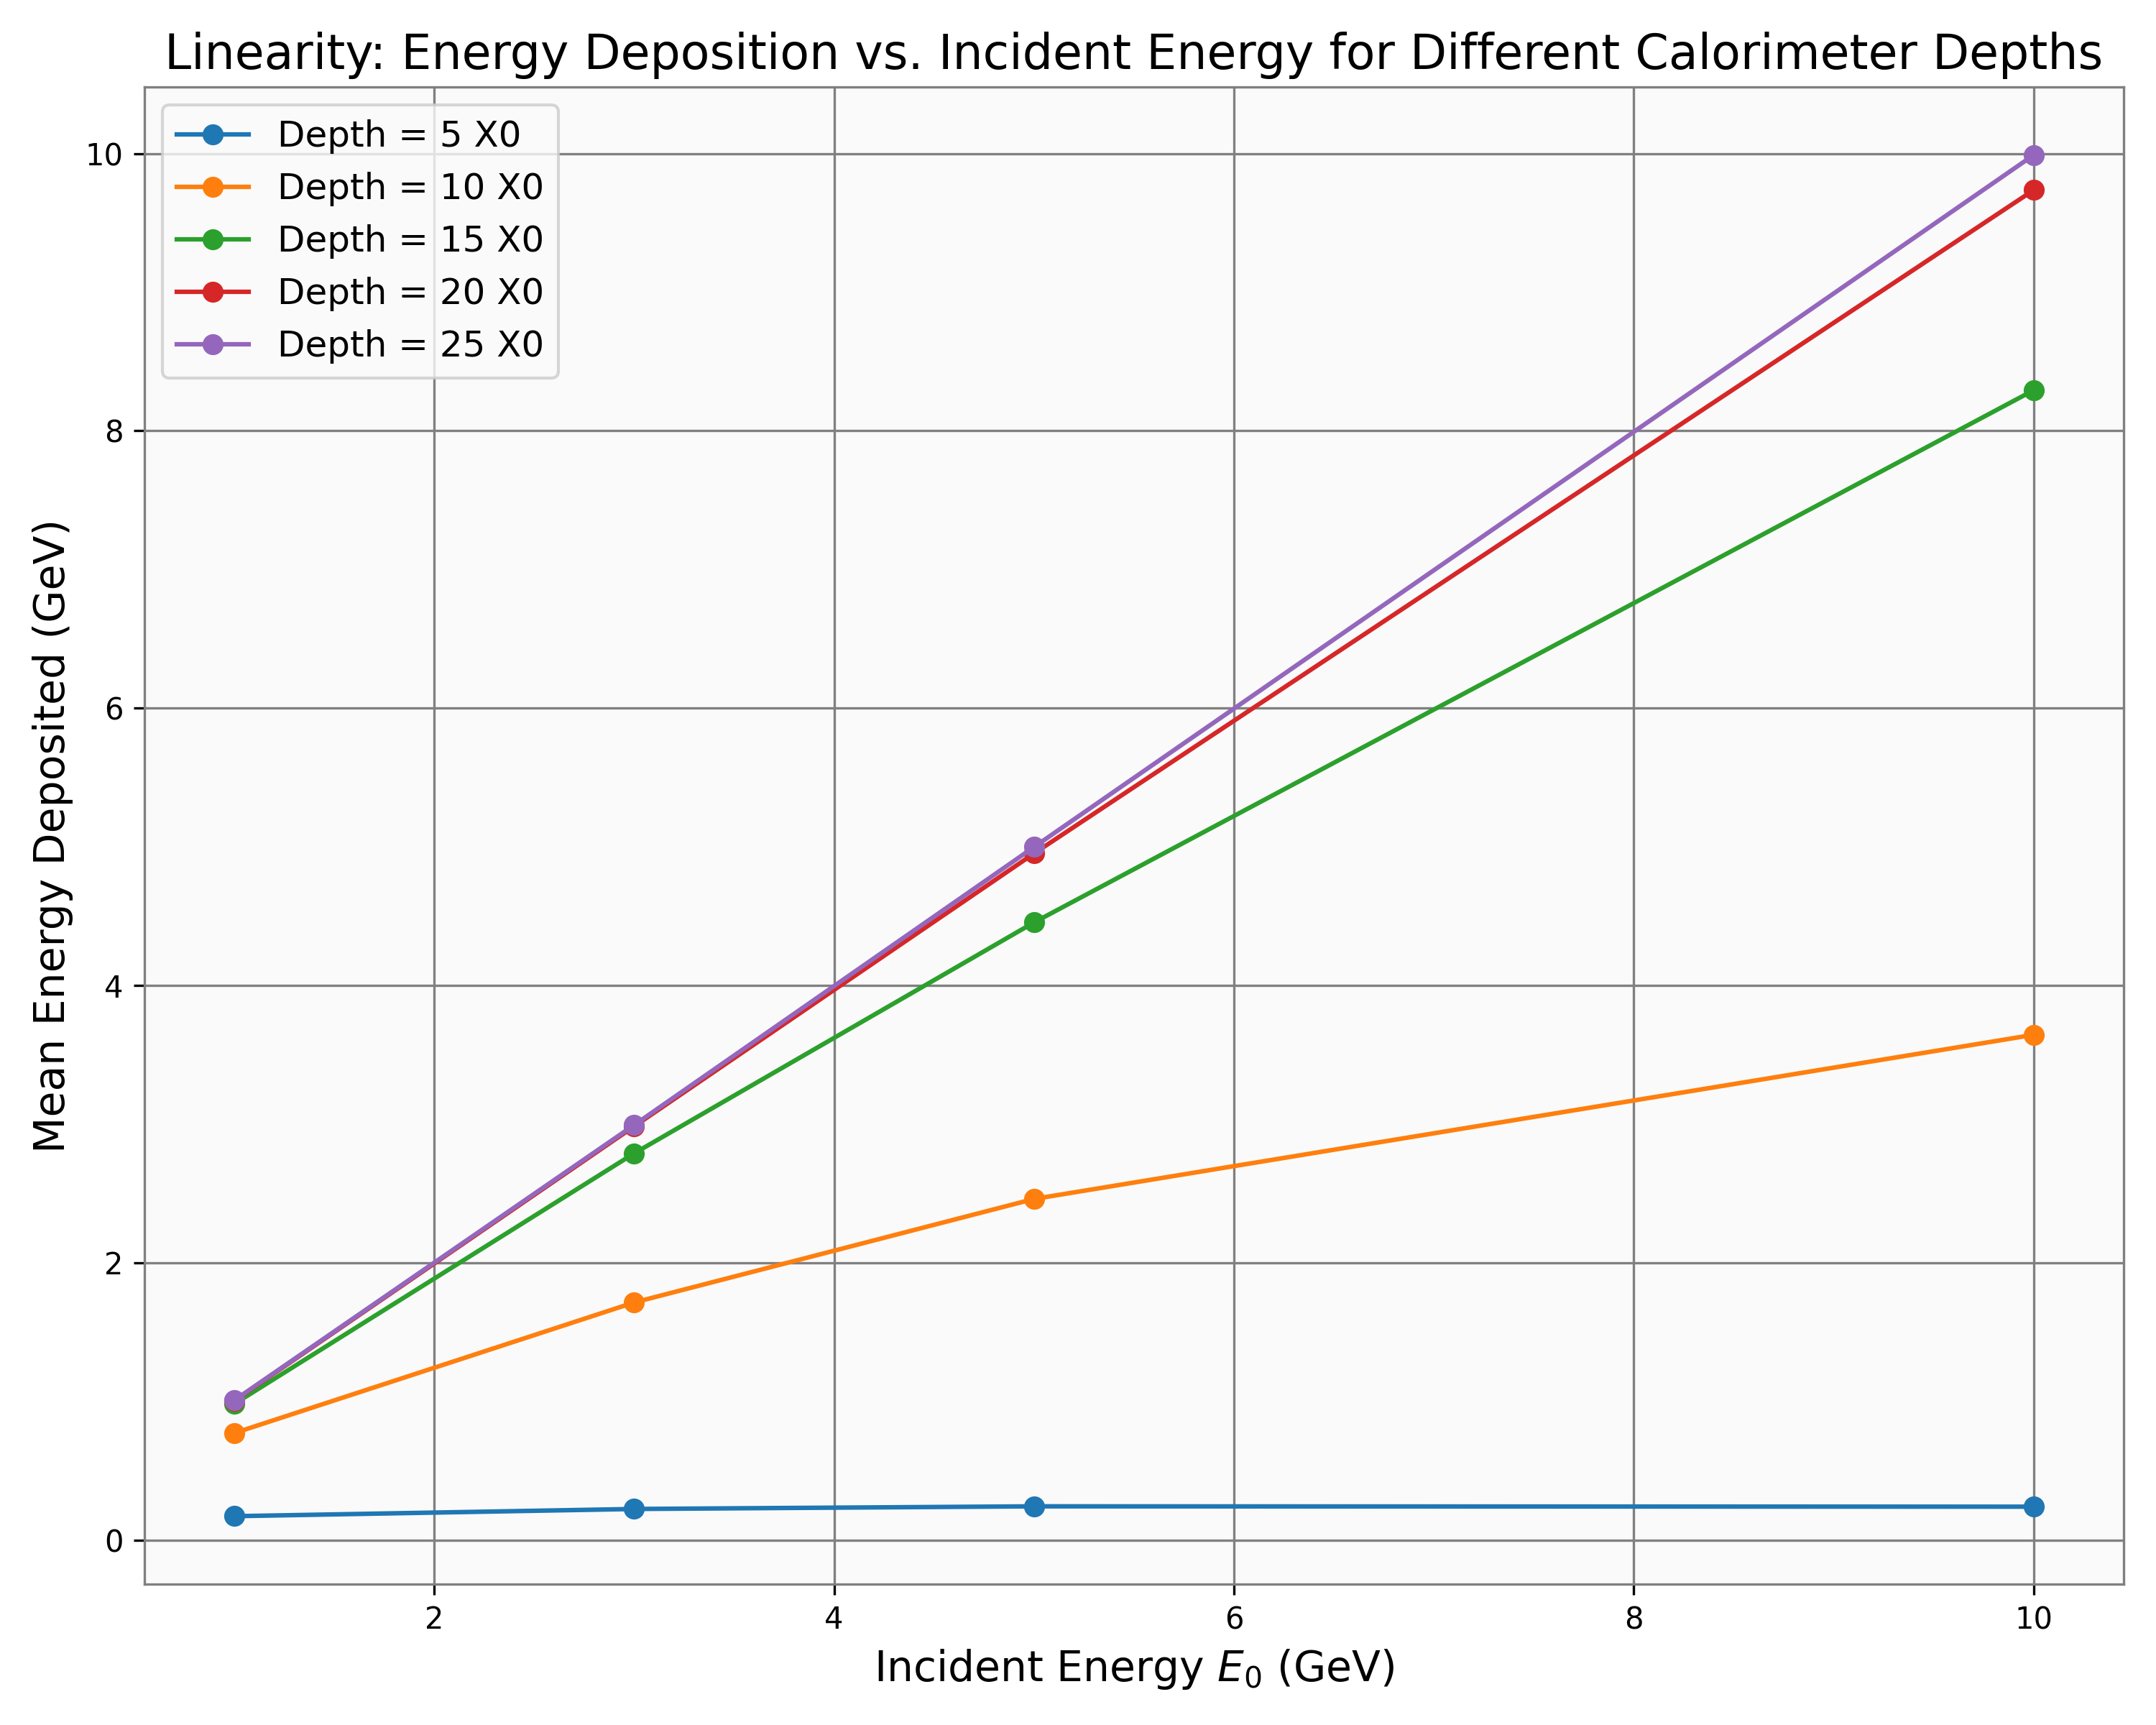
\includegraphics[width=\columnwidth]{linearity_vs_depth.png}
    \caption{Mean Energy Deposition (GeV) vs. Incident Energy \(E_0\) for calorimeter depths of 5, 10, 15, 20, and 25 \(X_0\). The plot illustrates how energy deposition approaches linearity with increasing calorimeter thickness.}
    \label{fig:mean_energy_deposition_depth}
\end{figure}

At a depth of 5 \(X_0\), the mean energy deposited remained nearly constant, ranging from 0.23 GeV at 1 GeV incident energy to 0.26 GeV at 10 GeV. Increasing the depth to 10 \(X_0\), the energy deposition followed a more square-root-like trend, with values increasing from 0.45 GeV at 1 GeV to 3.83 GeV at 10 GeV. Further increasing the depth to 15, 20, and 25 \(X_0\) resulted in an increasingly linear trend, with diminishing differences in energy deposition as the calorimeter becomes thicker.

\subsubsection{Linearity Ratio vs. Incident Energy}

The linearity ratio, defined as the mean energy deposited divided by the incident energy, was plotted against the incident energy for various calorimeter thicknesses.

\begin{figure}[htp]
    \centering
    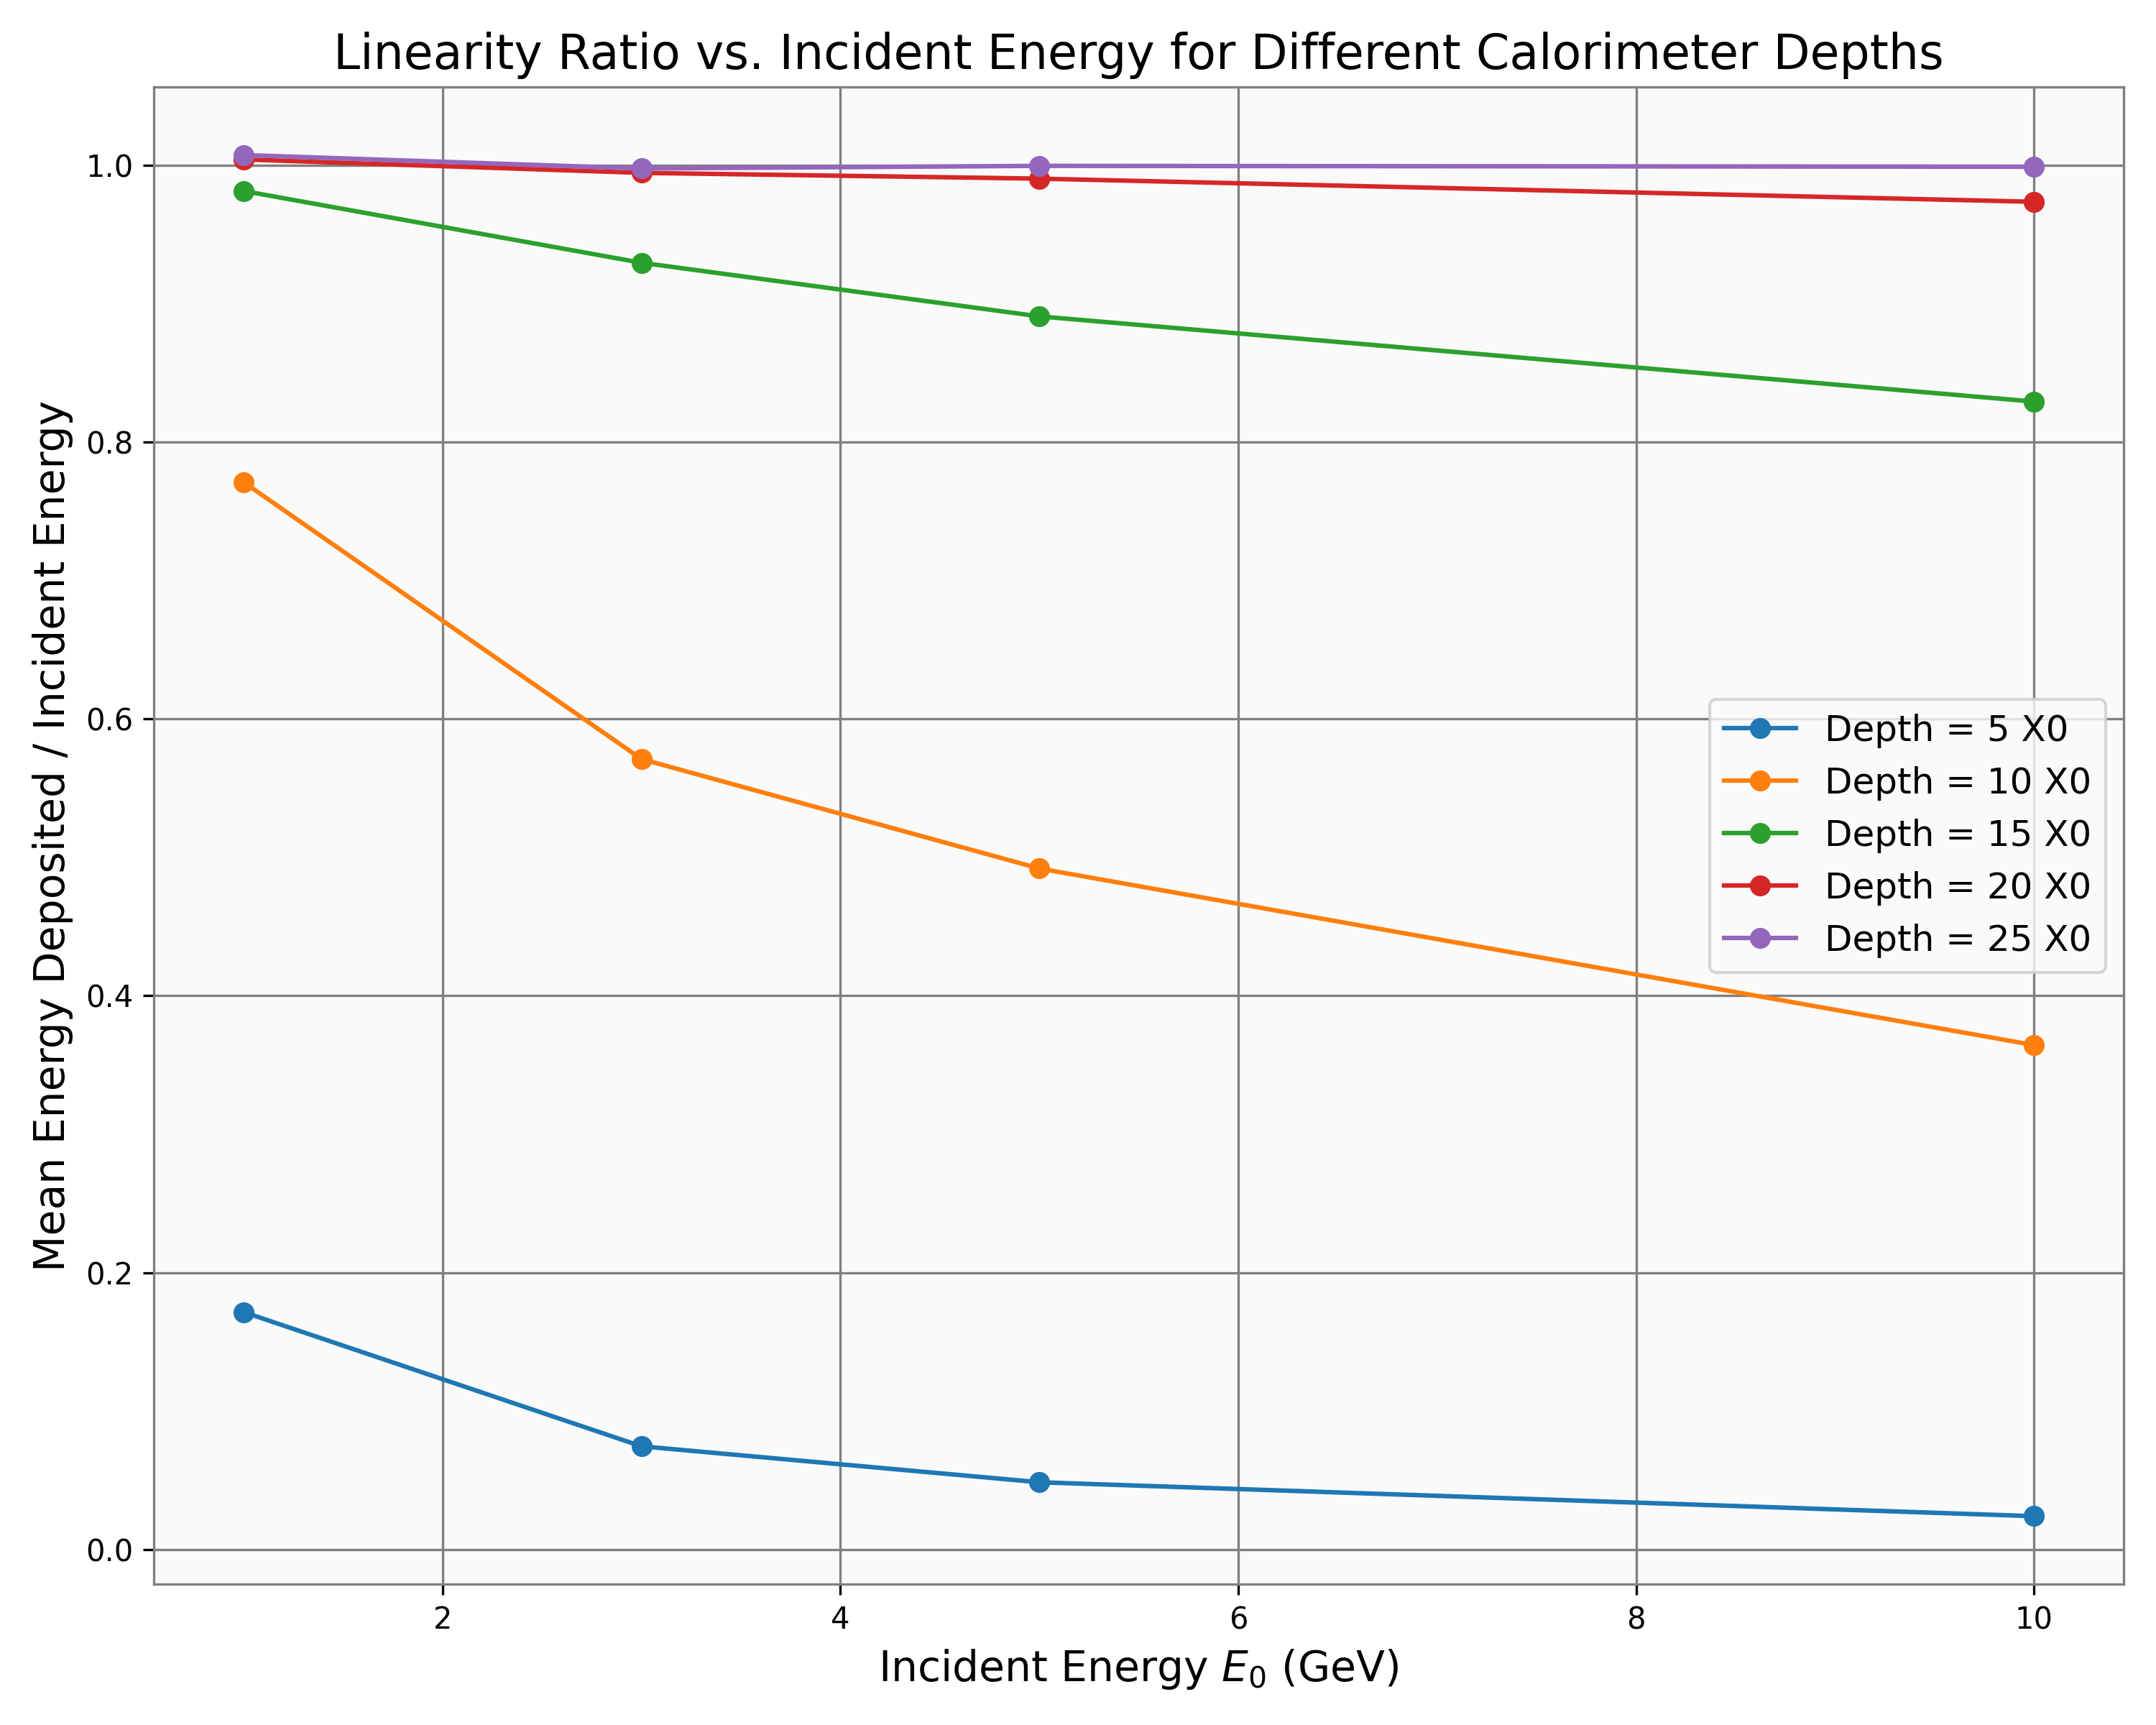
\includegraphics[width=\columnwidth]{linearity_ratio_vs_depth.png}
    \caption{Linearity ratio (Mean Energy Deposited / Incident Energy) vs. Incident Energy for different calorimeter depths. The plot shows the onset of non-linearities at lower depths and the stabilization of the linearity ratio at greater depths.}
    \label{fig:linearity_ratio_vs_depth}
\end{figure}

At a depth of 5 \(X_0\), the linearity ratio was approximately 0.183 at 1 GeV and decreased to 0.032 at 10 GeV, following an inverse square root trend that flattens with increasing incident energy. At 10 \(X_0\), the ratio was 0.779 at 1 GeV and 0.383 at 10 GeV, exhibiting a steeper trend. Deeper calorimeters (15, 20, and 25 \(X_0\)) showed reduced differences in linearity ratios across incident energies, with trends becoming more flat as thickness increases.

\subsubsection{Energy Resolution vs. Incident Energy for Varying Thicknesses}

The energy resolution, defined as the standard deviation of the energy deposition distribution, was evaluated for different calorimeter thicknesses.

\begin{figure}[htp]
    \centering
    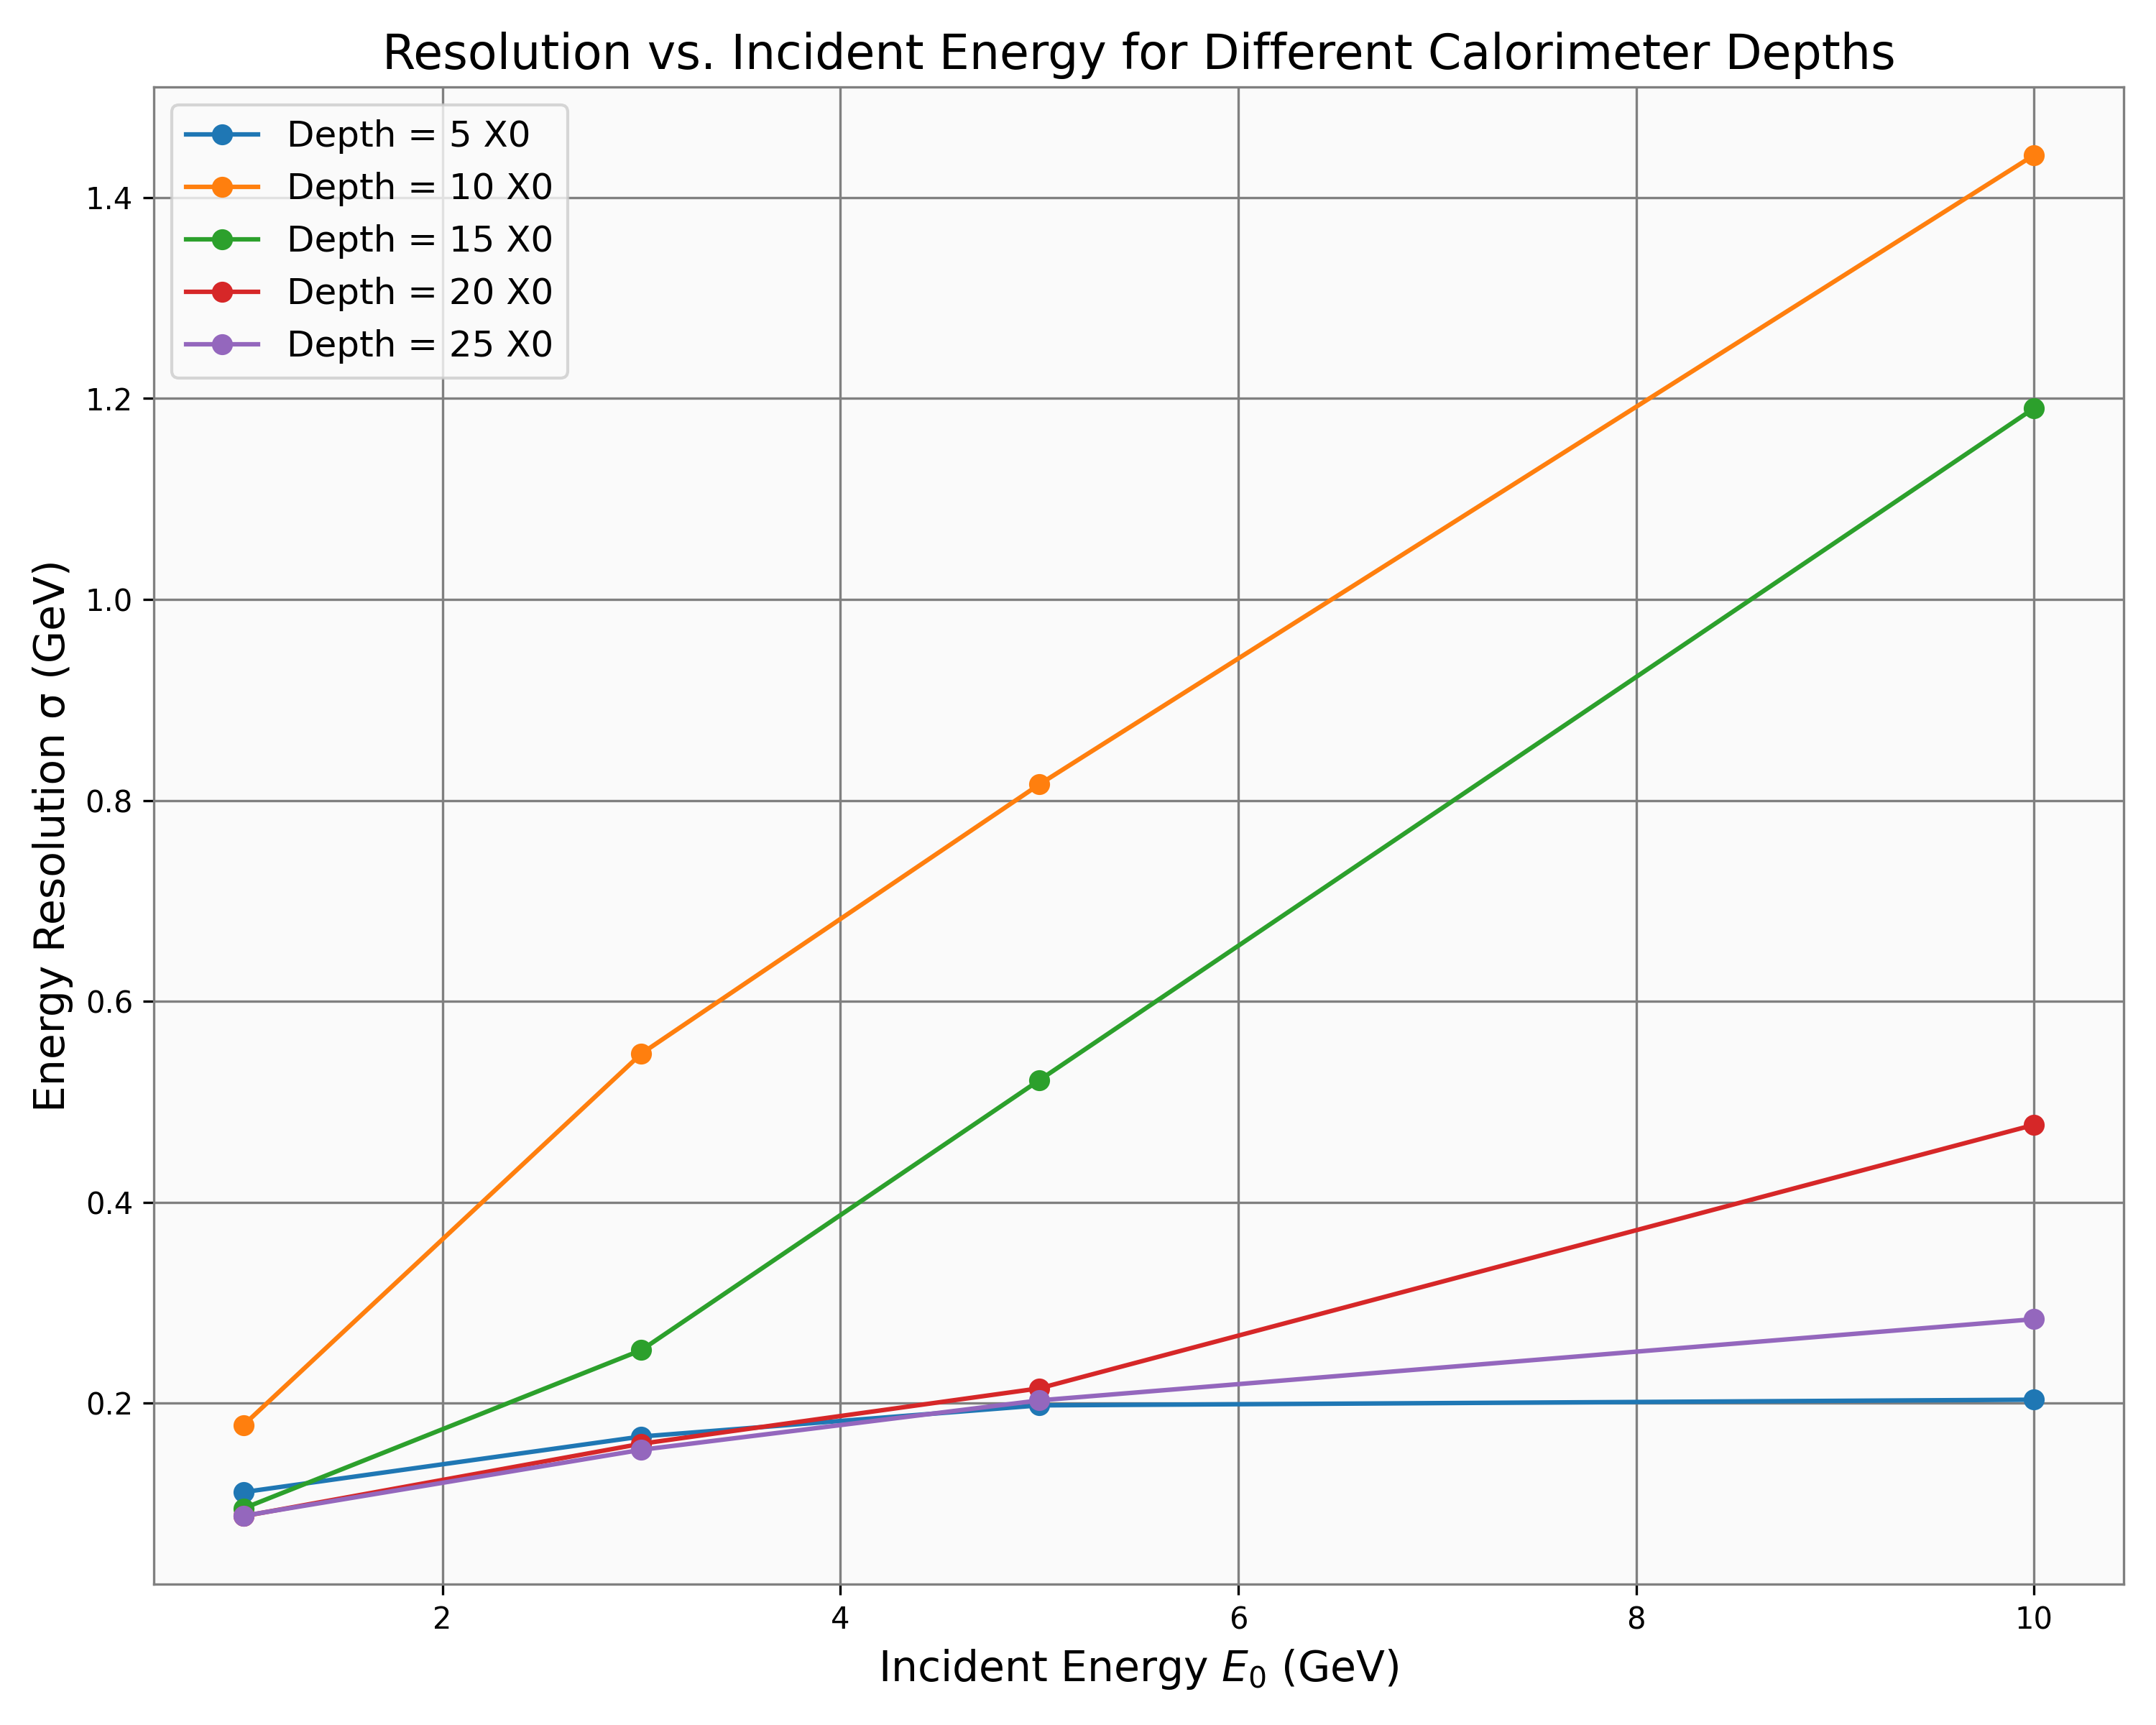
\includegraphics[width=\columnwidth]{resolution_vs_depth.png}
    \caption{Energy resolution (\(\sigma\)) vs. Incident Energy for different calorimeter depths. The resolution follows a square root trend for most depths, with some deviations at intermediate thicknesses.}
    \label{fig:resolution_vs_depth}
\end{figure}

For a calorimeter depth of 10 \(X_0\), the resolution followed a square root trend, similar to earlier phases. However, at 5 \(X_0\), the resolution was smaller but still adhered to a square root trend. At 15 \(X_0\), an unexpected quadratic trend emerged, likely due to the simulation's simplifying assumptions beyond the peak shower development. Depths of 20 and 25 \(X_0\) exhibited resolutions similar to 5 \(X_0\), with slight deviations towards an inverse square root trend, possibly resulting from the equal energy sharing and discrete interaction assumptions.

\subsubsection{Relative Energy Resolution vs. Incident Energy}

To better visualize the energy resolution, the relative energy resolution (\(\sigma/E\)) was plotted against incident energy for various calorimeter thicknesses.

\begin{figure}[htp]
    \centering
    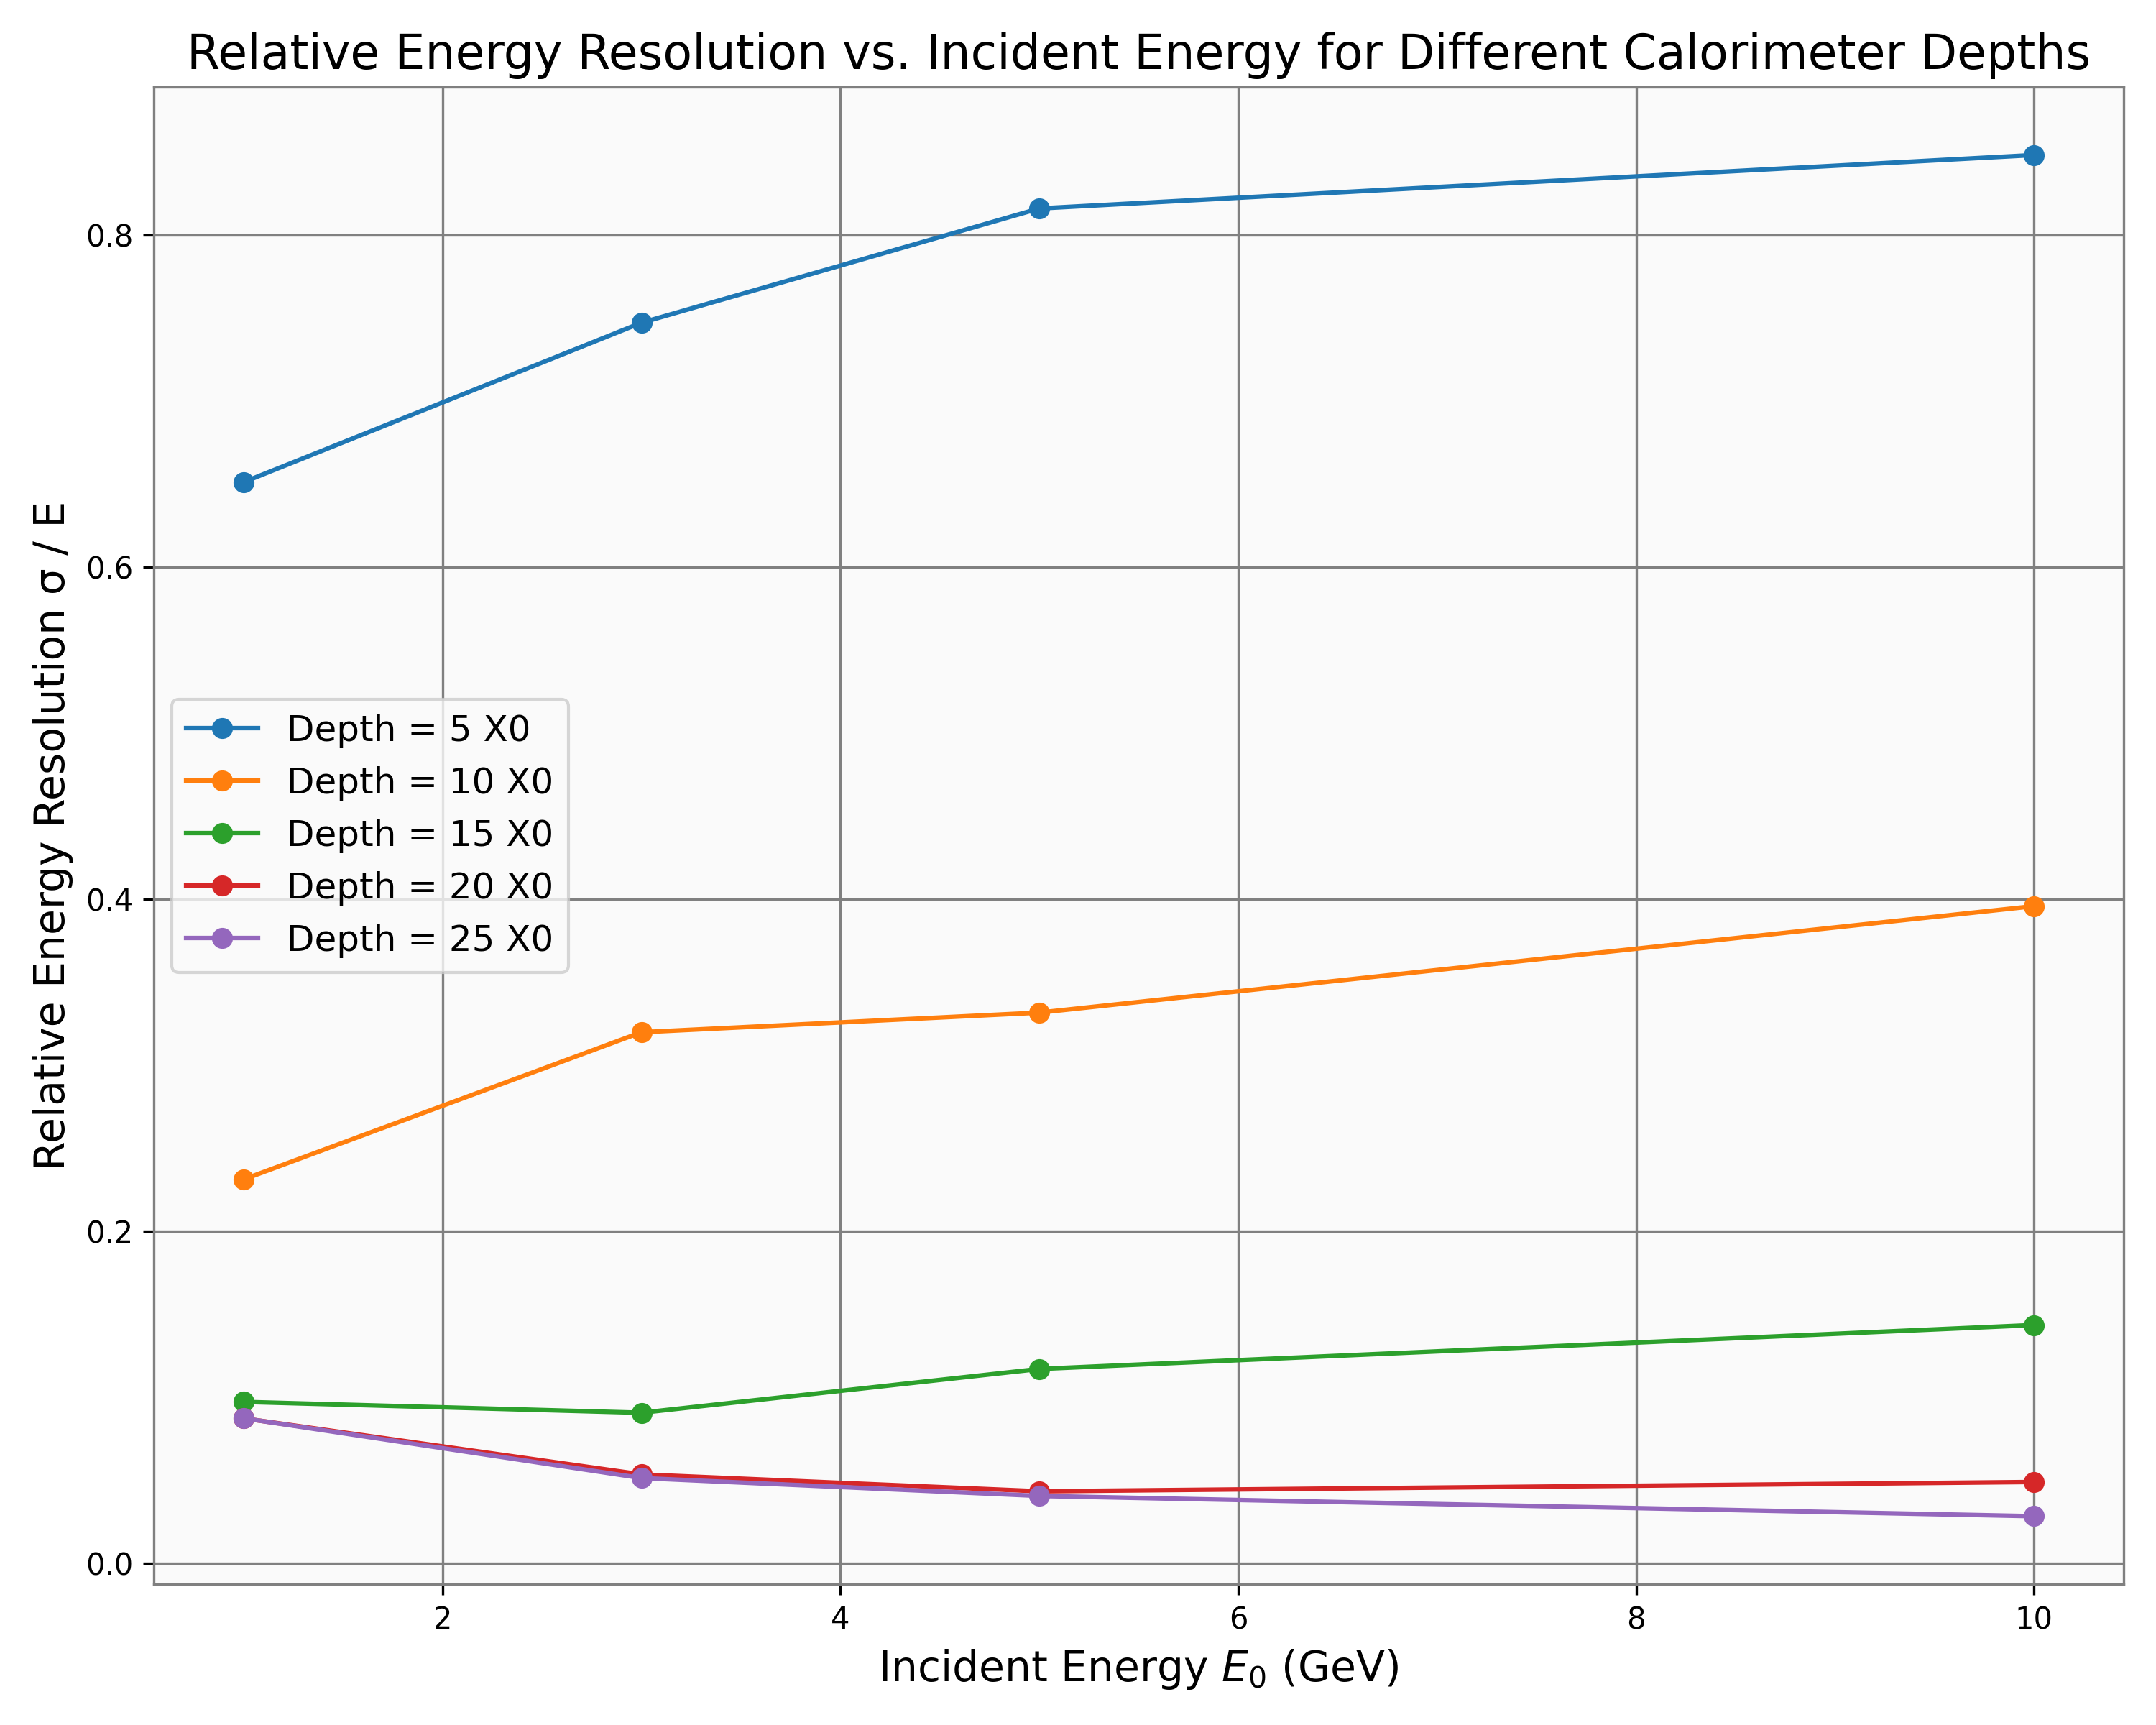
\includegraphics[width=\columnwidth]{relative_resolution_vs_depth.png}
    \caption{Relative energy resolution (\(\sigma/E\)) vs. Incident Energy for different calorimeter depths. The plot clarifies the scaling behavior, highlighting the square root dependence and the impact of calorimeter thickness on resolution.}
    \label{fig:relative_resolution_vs_depth}
\end{figure}

At 5 \(X_0\), the relative energy resolution was highest, following the expected square root trend. At 10 \(X_0\), the resolution was significantly lower but still adhered to the square root trend. Deeper calorimeters (15, 20, and 25 \(X_0\)) showed progressively smaller differences in relative energy resolution, with 20 and 25 \(X_0\) exhibiting trends that deviated slightly from the square root dependence, likely due to the simulation's simplifying assumptions.

\section{Results}\label{sec:results_phase1}

\subsection{Phase 1: Longitudinal Development of Electromagnetic Showers}

The Monte Carlo simulation was executed for 1000 events of 1 GeV electrons incident on a 25 cm deep PbWO\(_4\) calorimeter. The resulting longitudinal distribution of charged particles was plotted against the depth in centimeters from the front face of the calorimeter.

\begin{figure}[htp]
    \centering
    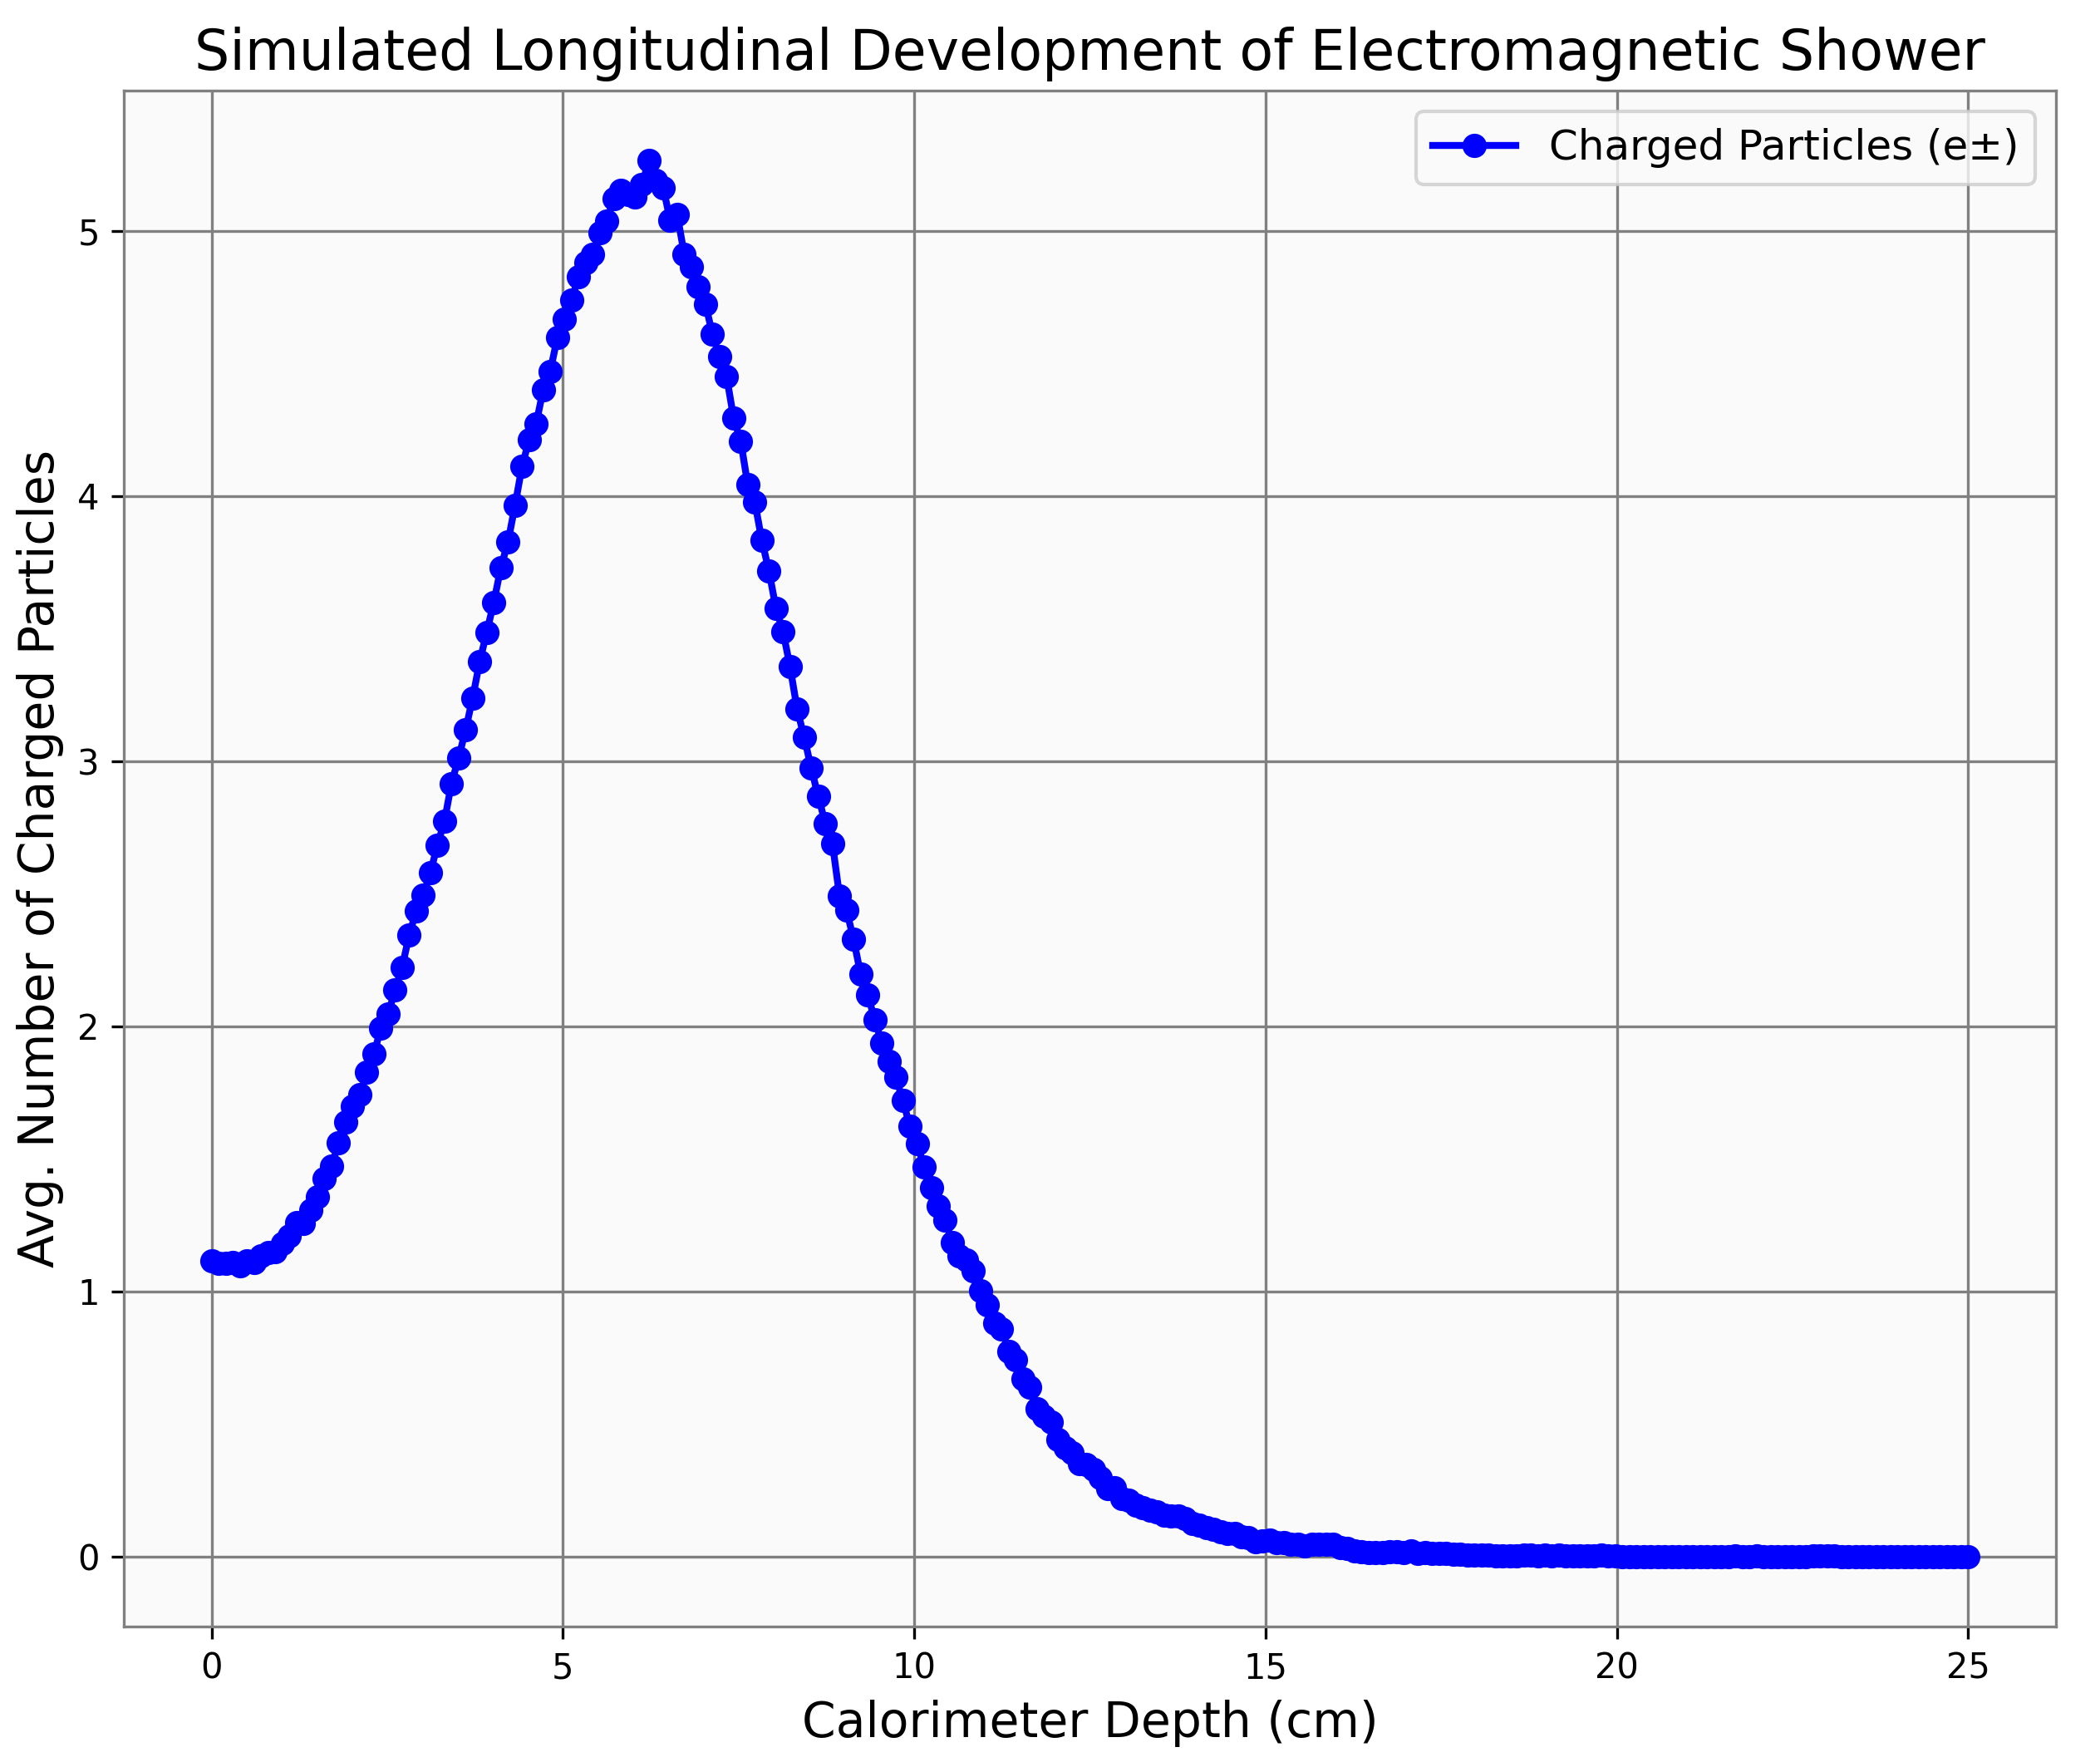
\includegraphics[width=\columnwidth]{part1_a.png}
    \caption{Average number of charged particles as a function of calorimeter depth for 1 GeV incident electrons. The distribution exhibits a peak at approximately 6.3 cm with around 9 charged particles crossing a plane at this depth. The shape closely resembles the charged particle distribution shown in PDG \textit{Passage of Particles Through Matter} Figure 33.20.}
    \label{fig:charged_particles_1GeV}
\end{figure}

\begin{figure}[htp]
    \centering
    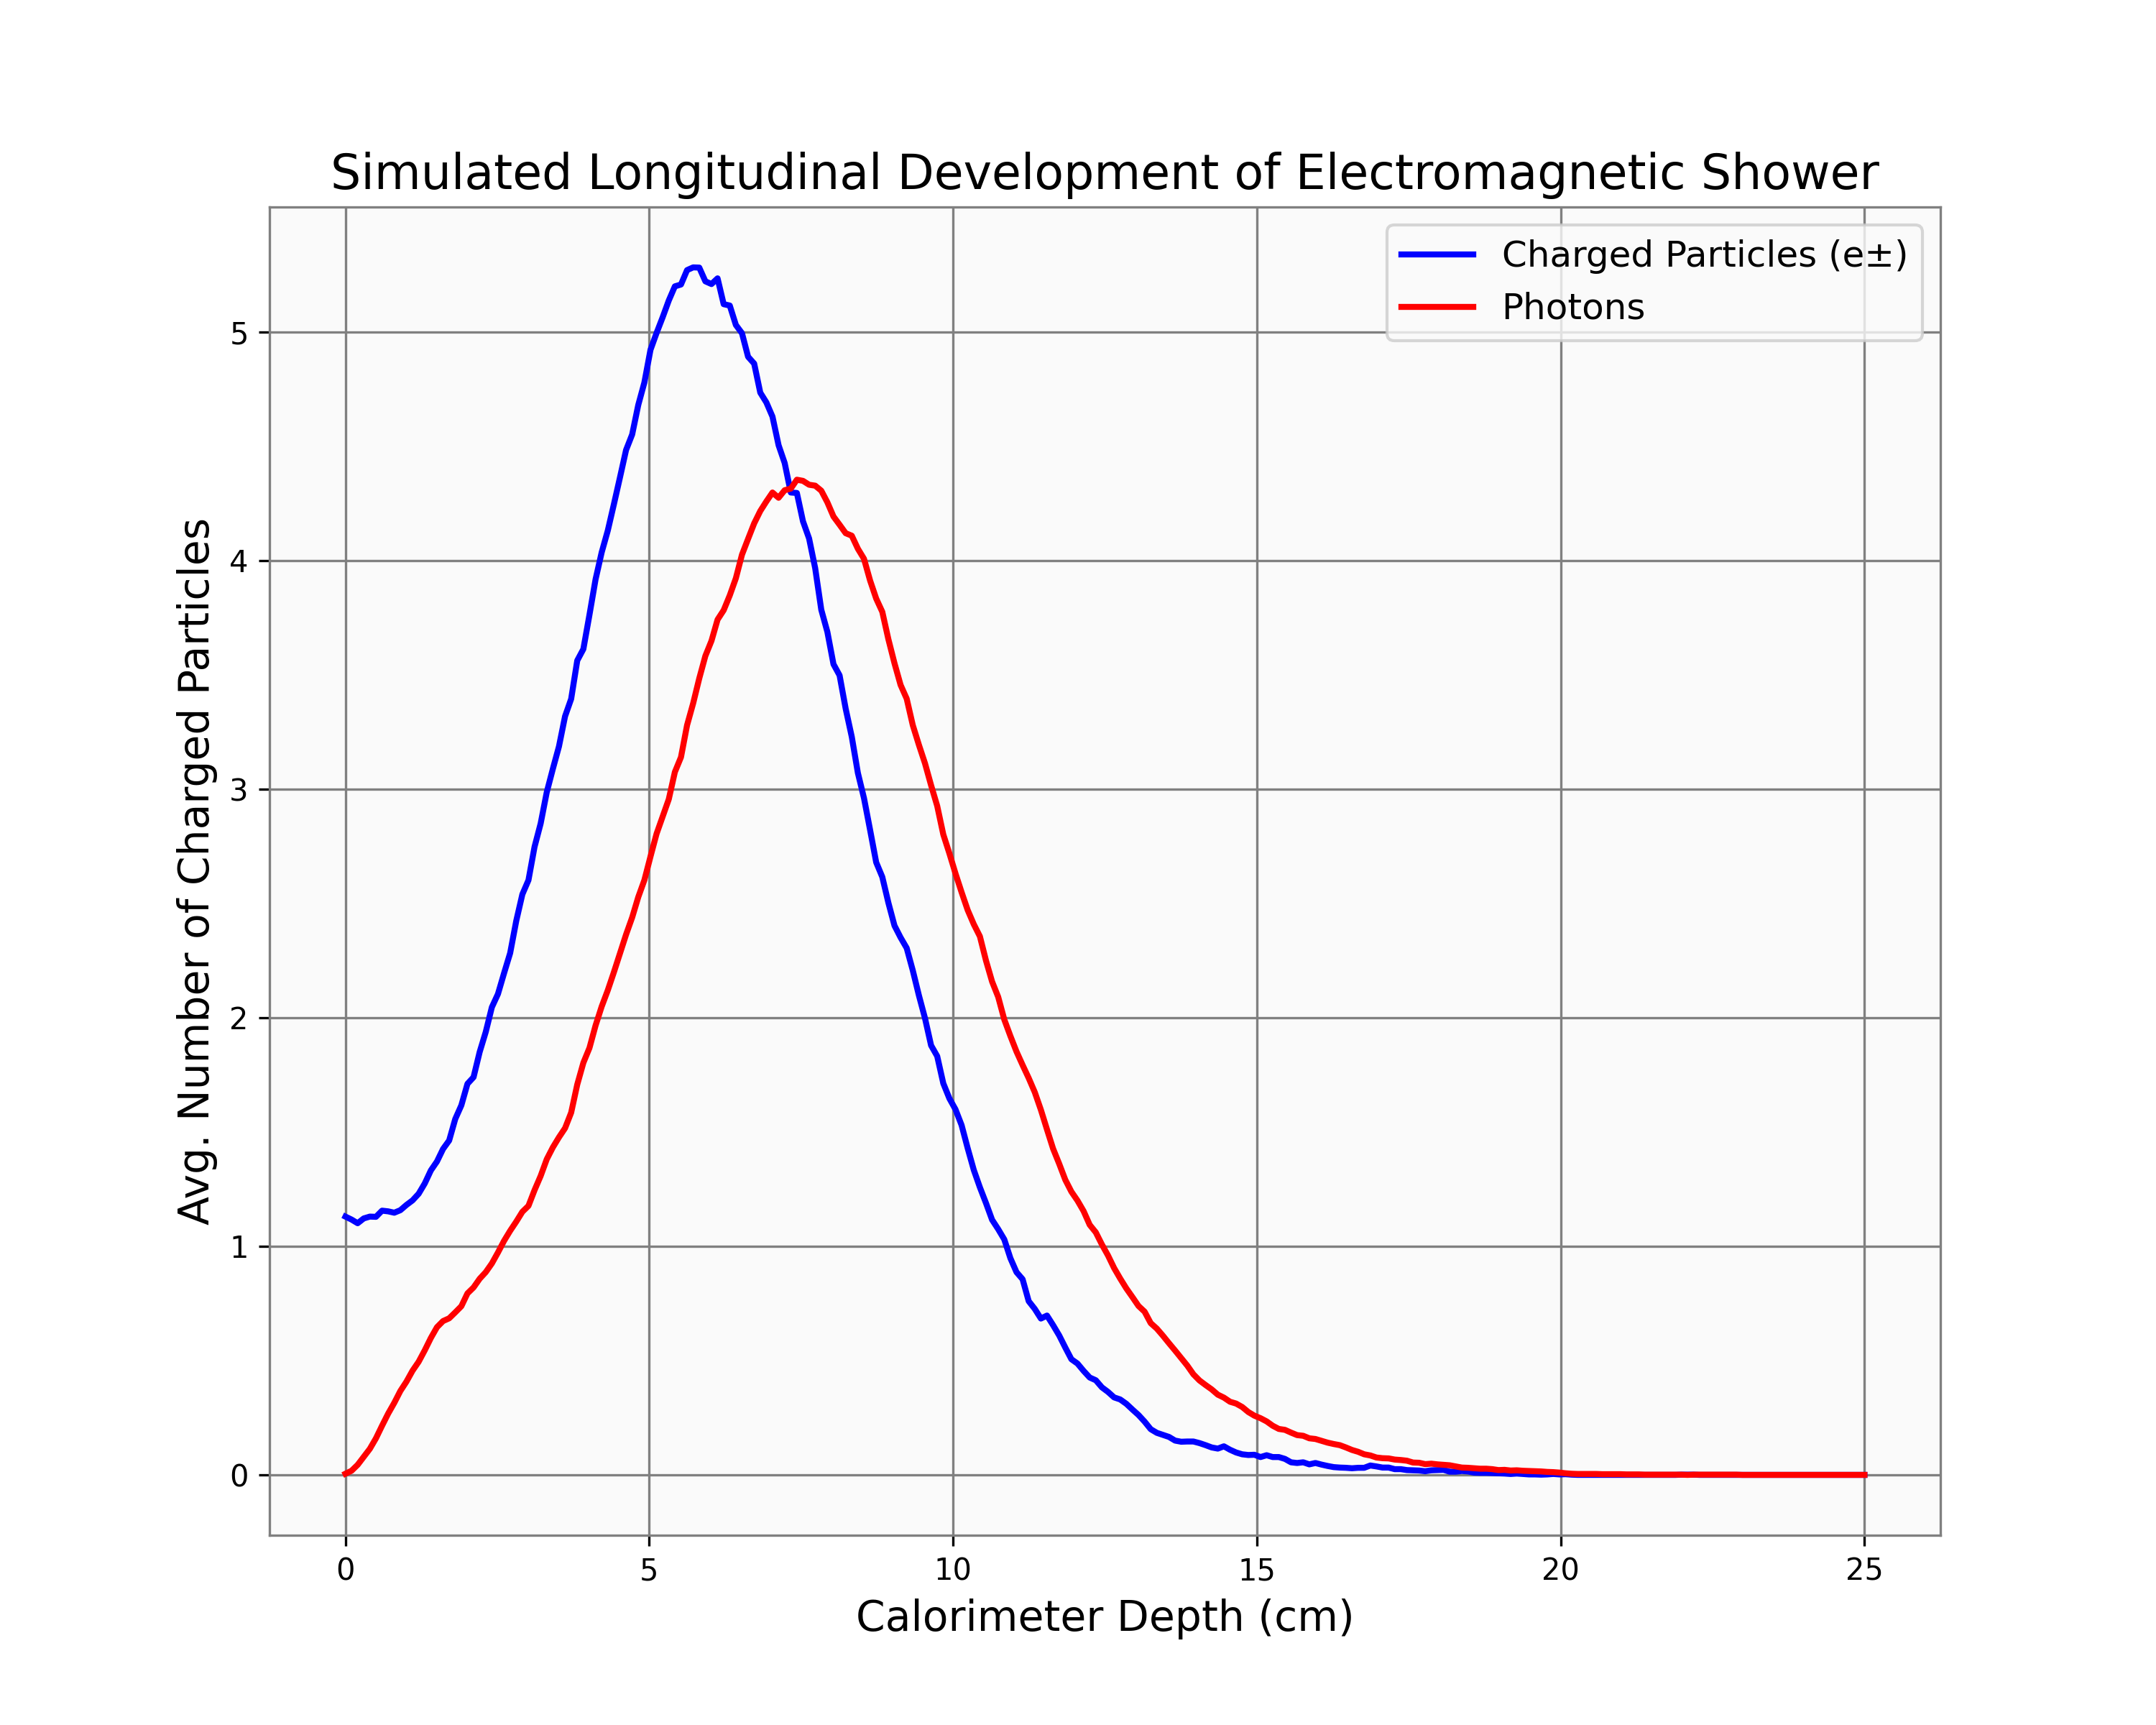
\includegraphics[width=\columnwidth]{part1_b.png}
    \caption{Comparison of average charged particle density and photon density as functions of calorimeter depth for 1 GeV incident electrons. Both distributions peak at similar depths, with the charged particle density surpassing the photon density prior to the peak, in agreement with PDG's simulation results.}
    \label{fig:charged_vs_photons_1GeV}
\end{figure}

\subsection{Phase 2: Linearity and Energy Resolution}

\subsubsection{Energy Deposition and Calibration}

The initial simulation with 1 GeV incident electrons resulted in a mean energy deposition of 3.027 GeV with a standard deviation of 0.263 GeV. Recognizing that this value was approximately three times the incident energy, a calibration factor of 1/3 was applied to align the mean energy deposition with the known incident energy. This calibration was validated across multiple incident energies, consistently yielding accurate mean values.

\subsubsection{Longitudinal Development at Multiple Energies}

Figure \ref{fig:charged_particles_multiple_energies} displays the average number of charged particles as a function of calorimeter depth for incident energies of 1, 3, 5, and 10 GeV. The results demonstrate that higher incident energies produce more charged particles and shift the shower maximum deeper into the calorimeter, maintaining a normal distribution shape.

\subsubsection{Energy Deposition vs. Incident Energy}

Figure \ref{fig:energy_deposition_vs_incident_energy} shows the linear relationship between incident energy and mean energy deposition in the calorimeter. The perfect linear fit (\(y = 1.00x + 0.00\)) indicates successful calibration under the simulation's simplifying assumptions.

\subsubsection{Energy Resolution Scaling}

Figure \ref{fig:energy_resolution_vs_energy} illustrates the calorimeter energy resolution as a function of incident energy. The resolution follows a square root dependence, fitting the relation \(\sigma = 0.09 \sqrt{E_0} - 0.007\), which is consistent with CMS reports. CMS typically observes that energy resolution scales as \(\sigma/E \propto \frac{1}{\sqrt{E}}\), reflecting the stochastic nature of the energy deposition processes in the calorimeter.

\subsection{Phase 3: Fitting the Energy Deposition Function}

Phase 3 involves fitting the energy deposition function to a gamma distribution to characterize the shower development. The parameters \(a\) and \(b\) were extracted for incident energies of 1, 3, 5, and 10 GeV, as summarized in Table \ref{tab:fitted_parameters}.

\begin{table}[htp]
    \centering
    \caption{Fitted parameters \(a\) and \(b\) for the energy deposition function at various incident energies.}
    \label{tab:fitted_parameters}
    \begin{tabular}{ccc}
        \hline
        \textbf{E\(_0\) (GeV)} & \textbf{a} & \textbf{b} \\
        \hline
        1 & 0.7991 & 0.0030 \\
        3 & 0.8622 & 0.0032 \\
        5 & 0.8784 & 0.0031 \\
        10 & 0.9400 & 0.0037 \\
        \hline
    \end{tabular}
\end{table}

These parameters indicate how the energy deposition profile evolves with increasing incident energy, reflecting changes in the shower development dynamics within the calorimeter.

\subsection{Phase 4: Linearity and Resolution vs. Calorimeter Thickness}

\subsubsection{Mean Energy Deposition vs. Incident Energy for Varying Thicknesses}

Figure \ref{fig:mean_energy_deposition_depth} showcases the mean energy deposition in GeV as a function of incident energy \(E_0\) for different calorimeter depths measured in radiation lengths (\(X_0\)). At a depth of 5 \(X_0\), the mean energy deposited remained nearly constant, ranging from 0.23 GeV at 1 GeV incident energy to 0.26 GeV at 10 GeV. Increasing the depth to 10 \(X_0\), the energy deposition followed a more square-root-like trend, with values increasing from 0.45 GeV at 1 GeV to 3.83 GeV at 10 GeV. Further increasing the depth to 15, 20, and 25 \(X_0\) resulted in an increasingly linear trend, with diminishing differences in energy deposition as the calorimeter becomes thicker.

\subsubsection{Linearity Ratio vs. Incident Energy}

Figure \ref{fig:linearity_ratio_vs_depth} presents the linearity ratio (Mean Energy Deposited / Incident Energy) as a function of incident energy for different calorimeter depths. At a depth of 5 \(X_0\), the linearity ratio was approximately 0.183 at 1 GeV and decreased to 0.032 at 10 GeV, following an inverse square root trend that flattens with increasing incident energy. At 10 \(X_0\), the ratio was 0.779 at 1 GeV and 0.383 at 10 GeV, exhibiting a steeper trend. Deeper calorimeters (15, 20, and 25 \(X_0\)) showed reduced differences in linearity ratios across incident energies, with trends becoming more flat as thickness increases.

\subsubsection{Energy Resolution vs. Incident Energy for Varying Thicknesses}

Figure \ref{fig:resolution_vs_depth} illustrates the energy resolution (\(\sigma\)) as a function of incident energy for different calorimeter depths. For a calorimeter depth of 10 \(X_0\), the resolution followed a square root trend, similar to earlier phases. However, at 5 \(X_0\), the resolution was smaller but still adhered to a square root trend. At 15 \(X_0\), an unexpected quadratic trend emerged, likely due to the simulation's simplifying assumptions beyond the peak shower development. Depths of 20 and 25 \(X_0\) exhibited resolutions similar to 5 \(X_0\), with slight deviations towards an inverse square root trend, possibly resulting from the equal energy sharing and discrete interaction assumptions.

\subsubsection{Relative Energy Resolution vs. Incident Energy}

Figure \ref{fig:relative_resolution_vs_depth} shows the relative energy resolution (\(\sigma/E\)) as a function of incident energy for different calorimeter depths. At 5 \(X_0\), the relative energy resolution was highest, following the expected square root trend. At 10 \(X_0\), the resolution was significantly lower but still adhered to the square root trend. Deeper calorimeters (15, 20, and 25 \(X_0\)) showed progressively smaller differences in relative energy resolution, with 20 and 25 \(X_0\) exhibiting trends that deviated slightly from the square root dependence, likely due to the simulation's simplifying assumptions.

\section{Conclusion}\label{sec:conclusion}

This study presents a Monte Carlo simulation of the longitudinal development of electromagnetic showers in the CMS electromagnetic calorimeter using a one-dimensional model.

\textbf{Phase 1} focused on simulating the shower profile for 1 GeV incident electrons in a 25 cm deep lead tungstate crystal, successfully replicating key features observed in established benchmarks, such as the PDG \textit{Passage of Particles Through Matter} Booklet's Figure 33.20. The peak charged particle density and its position within the calorimeter aligned with theoretical expectations, demonstrating the validity of the simulation approach despite the simplifying assumptions employed.

\textbf{Phase 2} extended the simulation to evaluate the detector's linearity and energy resolution across incident energies of 1, 3, 5, and 10 GeV. The calibration procedure effectively aligned the mean energy deposition with the known incident energies, and the results exhibited a perfect linear relationship between incident energy and measured energy deposition. Additionally, the energy resolution was found to scale with the square root of the incident energy, consistent with CMS reports.

\textbf{Phase 3} involved fitting the energy deposition function to a gamma distribution, extracting parameters \(a\) and \(b\) for various incident energies. The fitted parameters provide a quantitative characterization of the shower development and demonstrate how the energy deposition profile evolves with increasing energy.

\textbf{Phase 4} explored the detector's performance as a function of calorimeter thickness. The results indicated that thinner calorimeters (5 \(X_0\)) exhibit significant non-linearities in energy response and higher relative energy resolution. As the calorimeter depth increases to 10 \(X_0\) and beyond, the energy deposition approaches linearity, and the energy resolution improves, following expected scaling behaviors. These findings highlight the importance of calorimeter thickness in optimizing detector performance and minimizing non-linearities in energy measurements.

The simulation's agreement with PDG benchmarks and CMS expectations underscores its potential as a foundational tool for further studies. Future work will involve incorporating more realistic physical processes, such as continuous bremsstrahlung energy loss and transverse shower spreading, as well as extending the simulation to higher incident energies and different calorimeter materials. These enhancements aim to provide a more comprehensive understanding of the CMS ECAL's performance, contributing to more accurate energy measurements and improved particle identification in high-energy physics experiments.

\end{document}

